\chapter{El Espacio Afín}

\begin{definicion}[Espacio afín]
    Sea $\cc{A}\neq \emptyset$ un conjunto y $V(\bb{K})$ un espacio vectorial\footnote{Por norma general, usaremos $\bb{K}=\bb{R}$. De forma excepcional, podremos usar $\bb{K}=\bb{C}$.}. Diremos que $\cc{A}$ es un espacio afín si
    \Func{\exists~~\vec{\cdot}}{\cc{A}\times \cc{A}}{V}{(P,Q)}{\vec{PQ}}
    que cumple lo siguiente:
    \begin{enumerate}
        \item $\forall P,Q,R\in \cc{A}$, entonces $\vec{PQ}+\vec{QR}=\vec{PR}$

        \item Fijado $P\in \cc{A}$, existe una biyección
        \Func{\varphi_p}{\cc{A}}{V}{Q}{\vec{PQ}}

        Esta propiedad, por la definición de biyección tenemos:
        \begin{enumerate}
            \item Inyectividad: $\vec{PQ}=\vec{PR}\Longrightarrow Q=R$,
            \item Sobreyectividad: $\forall v\in V$, $\exists Q\mid \vec{PQ}=v$.
        \end{enumerate}
    \end{enumerate}

    A los elementos de $\cc{A}$ los llamaremos puntos, y a los elementos de $V$ los llamaremos vectores. Al espacio vectorial $V$ lo llamaremos espacio de direcciones de $\cc{A}$. Por ello, a veces notaremos $V=\vec{\cc{A}}$.
\end{definicion}

\begin{ejemplo}
    Los primeros ejemolos de espacios afines son los espacios vectoriales, como vamos a ver a continuación:
    \begin{enumerate}
        \item En $\bb{R}^3$, tenemos que la aplicación $\vec{\cdot}$ es:
        \Func{\vec{\cdot}}{\bb{R}^3\times \bb{R}^3}{\vec{\bb{R}^3}}{(P,Q)}{\vec{PQ}=Q-P}

        \item Para cualquier espacio vectorial $V(\bb{K})$, tenemos que la aplicación $\vec{\cdot}$ es:
        \Func{\vec{\cdot}}{V\times V}{V}{(u,v)}{\vec{uv}=v-u}

        Veamos las dos propiedades:
        \begin{enumerate}
            \item $\forall u,v,w\in V$, se tiene que:
            \begin{equation*}
                \vec{uv} + \vec{vw} = v-u+w-v = w-u = \vec{uw}
            \end{equation*}

            \item Fijado $v\in V$, tenemos la siguiente biyección:
            \Func{\varphi_v}{V}{V}{w}{w-v}
        \end{enumerate}

        Por este ejemplo, tenemos que todo espacio vectorial se puede ver como espacio afín, y decimos que es su \ul{estructura afín canónica}.
    \end{enumerate}
\end{ejemplo}


Algunas consecuencias de la definición de espacio afín son:
\begin{enumerate}
    \item $\vec{PQ}=\vec{0}\Longleftrightarrow Q=P$
    
    Suponemos $Q=P$. Entonces,
        $$\vec{PQ}+\vec{QP}=\vec{PP}+\vec{PP}=\vec{PP}\Longrightarrow \vec{PP}=\vec{0}$$

    Como tenemos que $\varphi_P$ es inyectiva, tenemos que ese punto es único, por lo que se da la doble implicación.
    
    \item $\vec{PQ}=-\vec{QP}$
    $$\vec{PQ}+\vec{QP}=\vec{PP}=\vec{0}$$

    \item Sean los puntos $P_1,\dots, P_k$. Entonces:
    $$\sum_{i=1}^{k-1}\vec{P_iP_{i+1}}=\vec{P_1P_k}$$

    Se demuestra fácilmente por inducción sobre $k$.

    \item Igualdad del paralelogramo: $\vec{P_1P_2}=\vec{Q_1Q_2}\Longrightarrow \vec{P_1Q_1}=\vec{P_2Q_2}$

    $$\vec{P_1Q_1}=\vec{P_1P_2} + \vec{P_2Q_1} = \vec{P_2Q_1} + \vec{Q_1Q_2} = \vec{P_2Q_2}$$
\end{enumerate}

Cabe destacar que podemos operar entre puntos y vectores considerando la inversa de la biyección descrita para el espacio afín:
\Func{\varphi_p^{-1}}{\vec{\cc{A}}}{\cc{A}}{v}{\varphi_p^{-1}(v)=Q}
donde tenemos que $\varphi_p^{-1}(v)=Q\Longleftrightarrow \vec{PQ}=v$. De tal forma, notamos $Q=P+v$ o, equivalentemente, $v=Q-P$. De esta notación, deducimos las siguientes propiedades:
\begin{enumerate}
    \item $\forall P\in \cc{A}$, tenemos que $P+\vec{0}=P$.
    \begin{equation*}
        P+\vec{0} = P+\vec{QQ} = P+Q-Q=P \hspace{1cm} \forall Q\in \cc{A}
    \end{equation*}
    \item $\forall P\in \cc{A}, u,v\in \vec{\cc{A}}$, se tiene que $P+(u+v)=(P+u)+v=R\in A$.
    
    Sean $Q=P+u$, $R=Q+v\in \cc{A}$. Entonces, $u=\vec{PQ},~v=\vec{QR}$, por lo que:
    \begin{equation*}
        P + (u+v) = P + \vec{PQ} + \vec{QR} = P + \vec{PR} = R = Q+v = (P+u)+v
    \end{equation*}

    \item Sean $P,Q,R\in \cc{A}, u,v\in \vec{\cc{A}}$ cumpliendo que:
    \begin{equation*}
        \begin{array}{rcl}
            P+u & = & Q  \\
            P+v & = & R
        \end{array}
    \end{equation*}
    Entonces, se tiene que $\vec{QR}=v-u$.

    \begin{equation*}
        \vec{QR} = R-Q = P+v-P-u = v-u
    \end{equation*}
\end{enumerate}


De las siguientes propiedades, podemos obtener el siguiente ejemplo de gran importancia:
\begin{ejemplo}\label{ej:espacio_afin_punto}
    Sea $\cc{A}=\{p\}$ un conjunto con un único punto. Entonces, tenemos que $\cc{A}$ es un espacio afín con:
        \Func{\vec{\cdot}}{\cc{A}\times \cc{A}}{\vec{\cc{A}}}{(p,p)}{\vec{0}}

        Veamos las dos propiedades:
        \begin{enumerate}
            \item $\forall p,q,r\in \cc{A}$, se tiene que $p=q=r$. Por tanto:
            \begin{equation*}
                \vec{pq} + \vec{qr} = \vec{0} + \vec{0} = \vec{0} = \vec{pr}
            \end{equation*}

            \item Fijado $p\in \cc{A}$, tenemos la siguiente biyección:
            \Func{\varphi_p}{\cc{A}}{\vec{\cc{A}}}{q}{\vec{pq}=\vec{0}}
        \end{enumerate}

        Además, como fijado $p\in \cc{A}$ tenemos que $\varphi_p$ es biyectiva
        y es constante en $\vec{0}$, tenemos que $\vec{\cc{A}}=\left\{\vec{0}\right\}$.
\end{ejemplo}


\begin{definicion}[Traslación]\label{def:traslacion}
    Dado un vector $v\in \vec{\cc{A}}$, definimos la traslación según $v$ de la siguiente forma:
    \Func{t_v}{\cc{A}}{\cc{A}}{p}{p+v}
\end{definicion}

Se tiene el siguiente resultado:
\begin{prop}
    Las traslaciones son movimientos biyectivos.
\end{prop}
\begin{proof}
    Sea $t_v$ la traslación a considerar.\\
    
    Demostremos en primer lugar que es inyectiva. Sean $P,Q\in \cc{A}$ tal que se cumple que $t_v(P)=t_v(Q)$. Entonces, $P+v=Q+v$, por lo que $P=Q$ y se tiene que es inyectiva.\\

    Veamos ahora que es sobreyectiva. $\forall Q\in \cc{A}$, $\exists P\in \cc{A}$ tal que $P+v=Q$ definiendo $P$ como $Q-v$.
\end{proof}

Algunas propiedades que se deducen directamente de la definición son:
\begin{enumerate}
    \item $t_{\vec{0}}=Id_{\cc{A}}$.
    \item $t_v\circ t_w = t_w\circ t_v = t_{v+w}$.
    \item $t_v\circ t_{-v}=Id_{\cc{A}}$
    \item $\{t_v\}_{v\in \vec{\cc{A}}}$ es un grupo abeliano.
\end{enumerate}


\begin{definicion}[Centro de Gravedad]
    Sea $\cc{A}$ un espacio afín con $\vec{\cc{A}}$. Sea una familia de puntos $P_1,\dots,P_k\in \cc{A}$, con $k\in \bb{N}$. Definimos el centro de gravedad o baricentro $G\in \cc{A}$ como
    $$G=O+\frac{1}{k}\sum_{i=1}^k \vec{OP_i}, \hspace{1cm} \forall O\in \cc{A}$$
\end{definicion}

Veamos que la definición no depende del punto $O$ escogido. Escogemos ahora $O'\in \cc{A}$ en vez de $O$. Entonces:
\begin{equation*}\begin{split}
    G&=O'+\frac{1}{k}\sum_{i=1}^k \vec{O'P_i}
    =O'+\frac{1}{k}\sum_{i=1}^k (\vec{O'O} + \vec{OP_i})
    = O' + \frac{k}{k}\vec{O'O} + \frac{1}{k}\sum_{i=1}^k \vec{OP_i}\\
    &= O' + O-O' + \frac{1}{k}\sum_{i=1}^k \vec{OP_i}
    = O+\frac{1}{k}\sum_{i=1}^k \vec{OP_i}
\end{split}\end{equation*}

Veamos el caso particular de $k=2$, que nos es de gran importancia por su interpretación geométrica.
\begin{definicion}[Punto medio]\label{def:PuntoMedio} Sea $\cc{A}$ un espacio afín. Entonces, dados dos puntos $p,q\in \cc{A}$, se define el punto medio entre los puntos $p$ y $q$ como el baricentro de dichos puntos. Es decir,
    \begin{equation*}
        m_{pq} = a + \frac{1}{2}(\vec{ap} + \vec{aq}) \qquad \forall a\in \cc{A}
    \end{equation*}

    Usando $a=p$, o $a=q$, tenemos:
    \begin{equation*}
        m_{pq} = p+\frac{1}{2}\vec{pq} = q + \frac{1}{2}\vec{qp}
    \end{equation*}
\end{definicion}
Notemos que, en el caso de que $\cc{A}$ sea un espacio euclídeo (se introducirá en el Tema \ref{chap:espacios_euclideos}), esta definición concuerda con la idea intuitiva de punto medio, ya que $d(p,m_{pq})=d(q,m_{pq})$.

\section{Subespacios afines}

\begin{comment}
\begin{ejemplo} Algunos ejemplos de espacios afines son:
\begin{enumerate}
    \item En $\bb{R}^2$ la recta $\cc{A}=\{(x,y)\mid x-y=-1\}$.
    
    Tenemos que su espacio de direcciones es $\vec{\cc{A}}=\{(x,y)\mid x=y\}$.
    
    \begin{figure}[H]
    \centering
    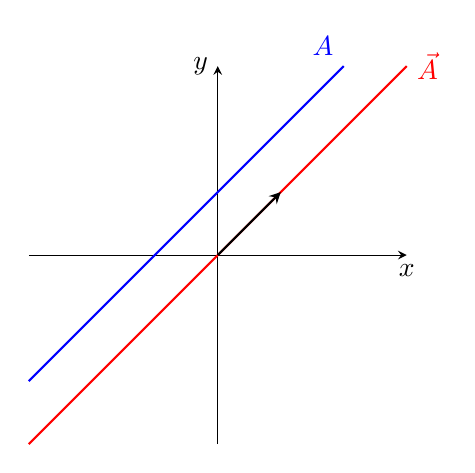
\begin{tikzpicture}[scale=0.8]
        % Eje x
        \draw[-stealth] (-3,0) -- (3,0) node[below] {$x$};
        % Eje y
        \draw[-stealth] (0,-3) -- (0,3) node[left] {$y$};

        % Recta x - y = -1 (Amarillo)
        \draw[thick, blue] (-3,-2) -- (2,3) node[above left] {$\cc{A}$};
        
        % Recta x = y (Rojo)
        \draw[thick, red] (-3,-3) -- (3,3) node[right] {$\vec{\cc{A}}$};
        
        % Vector desde el origen a (1,1)
        \draw[-stealth, thick] (0,0) -- (1,1);
    \end{tikzpicture}
    \end{figure}

    Sea $P=(x_1,y_1), Q=(x_2,y_2)\in \cc{A}$. Definimos $\vec{\cdot}:\cc{A}\times \cc{A}\to \cc{A}$ como:
    \begin{equation*}
        \vec{PQ} = (x_2-x_1, y_2-y_1)
    \end{equation*}
    
    Tenemos que es un espacio afín.

    \item En $\bb{R}^3$ el plano $F=\{(x,y,x)\mid ax+by+cz=d\}$ es un espacio afín.
    
    Su espacio de direcciones es $\vec{F}=\{(x,y,x)\mid ax+by+cz=0\}$.
\end{enumerate}
\end{ejemplo}
\end{comment}

\begin{definicion}[Subespacios afines]
    Sea $\cc{A}$ un espacio afín con $\vec{\cc{A}}$ espacio de direcciones.
    Un subconjunto $S\subseteq \cc{A}$ diremos que es un subespacio afín de $\cc{A}$ si $\exists p\in \cc{A}$
    y un subespacio vectorial $\vec{F}\subseteq \vec{\cc{A}}$ tal que $$S=p+\vec{F}=\left\{p+v\mid v\in \vec{F}\right\}$$

    A $\vec{F}$ lo llamaremos espacio de direcciones (o variedad de direcciones) de $S$.
\end{definicion}
Algunas propiedades de los subespacios afines son:
\begin{enumerate}
    \item $\vec{F}=\left\{\vec{PQ}\mid ~Q\in S\right\}$.
    \begin{description}
        \item[$\subset)$] Si $v\in \vec{F}$, entonces definimos $Q:=P+v\in S$. Por tanto, $v=Q-P=\vec{PQ}$, con $Q\in S$.

        \item[$\supset)$] Dado $Q\in S$, tenemos que $Q=P+\vec{PQ}\in S$, por lo que $\vec{PQ}\in \vec{F}$.
    \end{description}
    \item $\vec{F}=\left\{\vec{P_1P_2}\mid P_1,P_2\in S\right\}$
    $$\vec{P_1P_2} = \vec{P_1P} + \vec{PP_2}\in \vec{F}$$
    \item(Unicidad del espacio de direcciones) Consideramos $F', F''$ subespacios vectoriales de $\vec{F}$. Entonces,
    $$Q+F' = P+F'' = S \Longrightarrow F'=F''$$
    de ahí, que denotemos $\vec{F}=\vec{S}$ y, por tanto,
    $$S=p+\vec{S}$$
\end{enumerate}

Veamos el siguiente resultado de gran importancia, que nos permite trabajar con los subespacios afínes
con las mismas propiedades que los espacios afínes.
\begin{prop}
    Sea $\cc{A}$ un espacio afín y sea $S=p+\vec{S}$ un subespacio afín. Entonces,
    $S$ es un espacio afín.
\end{prop}
\begin{proof}
    Tenemos que todo punto de $S$ se puede escribir como $p+v$ con $v\in \vec{S}$. Por tanto, se define $\vec{\cdot}$ como:
    \Func{\vec{\cdot}}{S\times S}{\vec{S}}{(p+v,p+w)}{w-v}

    Veamos que cumple las propiedades de espacio afín:
    \begin{enumerate}
        \item $\vec{PQ}+\vec{QR}=\vec{PR}$

        Sean $P=p+v,~Q=p+w,~R=p+z\in S$. Entonces,
        \begin{equation*}
            \vec{PQ}+\vec{QR} = w-v+z-w = z-v = \vec{PR}
        \end{equation*}

        \item Fijado $P=p+v\in S$, tenemos la siguiente biyección:
        \Func{\varphi_P}{S}{\vec{S}}{Q=p+w}{w-v}

        Veamos que es inyectiva. Sean $Q_1=p+w_1, Q_2=p+w_2\in S$ tal que $\varphi_P(Q_1)=\varphi_P(Q_2)$. Entonces, $w_1-v=w_2-v$, por lo que $w_1=w_2$ y se tiene que es inyectiva.\\

        Veamos ahora que es sobreyectiva. $\forall w\in \vec{S}$, $\exists Q\in S$ tal que $\varphi_P(Q)=w$ definiendo $Q$ como $p+w$.
    \end{enumerate}
\end{proof}


\begin{definicion}
    La dimensión de un espacio afín $\cc{A}$ es la dimensión de su variedad de direcciones
    $$\dim \cc{A} :=\dim \vec{\cc{A}}$$
    
    A veces, lo notaremos como $\cc{A}^n$, con $n=\dim \cc{A}$.
\end{definicion}

Algunos subespacios afines $S\subset \cc{A}$ con determinadas dimensiones tienen nombre concreto, que son:
\begin{itemize}
    \item $\dim S=0$: Punto.
    \item $\dim S=1$: Recta.
    \item $\dim S=2$: Plano.
    \item $\dim S=\dim \cc{A}-1$: Hiperplano.
\end{itemize}

\begin{prop}
    Dados $P,Q\in \cc{A}$, $P\neq Q$, tenemos que $\exists_1$ recta $r$ tal que $P,Q\in r$.
\end{prop}
\begin{proof}
    El espacio de direcciones es $\vec{r}=\cc{L}\left(\vec{PQ}\right)$. Por tanto, tenemos que existe una recta $r=P+\cc{L}\left(\vec{PQ}\right)$.

    Supongamos que existe otra recta $r'=P+\cc{L}(v)$. Como $\vec{PQ}\in \vec{r'}$, entonces podemos tomar $\cc{L}(v)=\cc{L}\left(\vec{PQ}\right)$, por lo que tienen la misma variedad de direcciones y, por tanto, es la misma recta.
\end{proof}


\subsubsection{Operaciones con subespacios afines}
\begin{prop}[Intersección]
    Sea $\cc{A}$ espacio afín. Consideramos $\{S_i\}_{i\in I}$ una familia de subespacios afines de $\cc{A}$. Si $\bigcap\limits_{i\in I}S_i\neq \emptyset$, se tiene que $\bigcap\limits_{i\in I}S_i$ es un subespacio afín con variedad de direcciones
    \begin{equation*}
        \vec{\bigcap\limits_{i\in I}S_i} = \bigcap\limits_{i\in I}\vec{S_i}
    \end{equation*}
\end{prop}
\begin{proof}
    Como $\bigcap\limits_{i\in I}S_i\neq \emptyset$, sea $p\in \bigcap\limits_{i\in I}S_i$. Demostremos que $\bigcap\limits_{i\in I}S_i=p+\bigcap\limits_{i\in I}\vec{S_i}$.

    \begin{description}
        \item[$\subset$)]
        Tomamos $q\in \bigcap\limits_{i\in I}S_i$, por lo que $\vec{pq}\in \bigcap\limits_{i\in I}\vec{S_i}$. Por tanto, queda demostrada esta inclusión.
        
        \item[$\supset$)] Sea $q\in p+\bigcap\limits_{i\in I}\vec{S_i}$. Entonces, $q=p+v$ con $v\in \bigcap\limits_{i\in I}\vec{S_i}$. Por tanto, $q\in S_i,~\forall i\in I$ y, por consiguiente, $q\in \bigcap\limits_{i\in I}S_i$.
    \end{description}
\end{proof}


\begin{definicion}[Suma afín]
    Sea $\cc{A}$ espacio afín. Consideramos $S,T$ subespacios afines.
    Llamamos suma afín de $S$ y $T$ (o subespacio afín generado por $S$ y $T$), denotado por $S\vee T$, al subespacio afín más pequeño que contiene a $S$ y $T$.
\end{definicion}

De la propia definición se deduce la forma de calcularla:
$$\Gamma=\{F\subset \cc{A}\mid F \text{ subespacio afín de } \cc{A} ~\land~ (S\cup T)\subset F\}$$
$$\bigcap_{F\in \Gamma} F = S\vee T$$

Además, $S\vee T$ es un espacio afín ya que es una intersección no vacía, ya que $(S\cup T)\subset (S\vee T)$.

\begin{prop}
    Sea $\cc{A}$ espacio afín. Consideramos $S,T$ subespacios afines dados por $S=p+\vec{S}$, $T=q+\vec{T}$. Tenemos que
    $$S\vee T = p+\left[\cc{L}\left(\vec{pq}\right) + \vec{S} + \vec{T}\right]$$
\end{prop}
\begin{proof}Definimos previamente $X:=p+\left[\cc{L}\left(\vec{pq}\right) + \vec{S} + \vec{T}\right]=p+\vec{X}$. Veamos que $S\vee T=X$.
    \begin{description}
        \item[$\subset$)] 
            Como $\vec{S}\subset \cc{L}\left(\vec{pq}\right) + \vec{S} + \vec{T}=\vec{X}$ y $p\in S$ (y por tanto en $X$), tenemos que:
            \begin{equation*}
                S=p+\vec{S}\subset p+ \vec{X} = X
            \end{equation*}

            Como $\vec{T}\subset \cc{L}\left(\vec{pq}\right) + \vec{S} + \vec{T}=\vec{X}$ y $q\in T$ (y por tanto en $X$), tenemos que:
            \begin{equation*}
                T=q+\vec{T}\subset q+ \vec{X} = p+ \vec{X} = X
            \end{equation*}

            Como $S,T\subset X$, entonces $S\vee T\subset X$ por ser $S\vee T$ el subespacio afín más pequeño que contiene a $S$ y $T$.
            
        \item[$\supset$)] Veamos que $\vec{X}\subset \vec{S\vee T}$.

        Como $S,T\subset S\vee T$, entonces $\vec{S},\vec{T}\subset \vec{S\vee T}$, por lo que $\vec{S}+\vec{T}\subset \vec{S\vee T}$.
        
        Además, como $p,q\in S\cup T\subset S\vee T$, tenemos que $\vec{pq}\in \vec{S\vee T}$, por lo que $\cc{L}\{\vec{pq}\}\subset \vec{S\vee T}$.

        Por tanto, $\vec{X}\subset \vec{S\vee T}$. Además, como $p\in S$, tenemos que $p\in S\vee T$. Por tanto, se tiene que $X\subset S\vee T$.
    \end{description}
\end{proof}

\begin{notacion}
    Sea $\cc{A}$ un espacio afín, y consideramos $q_0,\dots,q_k\in \cc{A}$. Definimos el subespacio afín generado por los puntos $\{q_i\}$ como:
    \begin{equation*}
        \bigvee_{i=0}^k \{q_i\} = \langle q_0,\dots,q_k \rangle
    \end{equation*}
\end{notacion}


\begin{prop}\label{prop:IntersecNoVacia}
    Sea $\cc{A}$ espacio afín. Consideramos $S,T$ subespacios afines dados por $S=p+\vec{S}$, $T=q+\vec{T}$. Tenemos que
    $$S\cap T\neq \emptyset \Longleftrightarrow \vec{pq}\in \left(\vec{S}+\vec{T}\right)$$
\end{prop}
\begin{proof}\
    \begin{description}
        \item[$\Longrightarrow)$] Sea $p_0\in S\cap T$. Entonces, $\vec{p_0p}\in \vec{S}$ y $\vec{p_0q}\in \vec{T}$. Por tanto,
        $$\vec{pq}=\vec{p_0p}+\vec{p_0q}\in (\vec{S}+\vec{T})$$

        \item[$\Longleftarrow)$] Como $\vec{pq}\in (\vec{S}+\vec{T})$, considerando $u\in \vec{S}$ y $v\in \vec{T}$ tenemos que $\vec{pq}=u+v$. Entonces, $q=p+\vec{pq}=p+u+v$. Entonces, $q-v\in T$ y $p+u\in S$, por lo que $q-v=p+u\in S\cap T$.
    \end{description}
\end{proof}
\begin{coro}
    Sea $\cc{A}$ espacio afín. Consideramos $S,T$ subespacios afines. Se tiene que
    $$\vec{S\vee T} = \vec{S} + \vec{T} \Longleftrightarrow S\cap T\neq \emptyset$$
\end{coro}



\begin{teo}[Dimensiones]
    Sea $\cc{A}$ espacio afín. Consideramos $S,T$ subespacios afines de $\cc{A}$ de dimensión finita. Entonces, tenemos que:
    \begin{itemize}
        \item Si $S\cap T\neq \emptyset$, entonces,
        \begin{equation*}
            \dim \left(S\vee T\right)+\dim (S\cap T)= \dim S + \dim T
        \end{equation*}

        \item Si $S\cap T= \emptyset$, entonces,
        \begin{equation*}
            \dim (S\vee T)+\dim\left(\vec{S} \cap \vec{T}\right)=\dim S + \dim T +1
        \end{equation*}
    \end{itemize}
\end{teo}
\begin{proof} Distinguimos para cada caso:
    \begin{itemize}
        \item Si $S\cap T\neq \emptyset$, entonces tenemos que es un subespacio afín. Además,
    \begin{equation*}\begin{split}
            \dim (S\cap T)
            &=\dim\left(\vec{S\cap T}\right)
            = \dim\left(\vec{S}\cap \vec{T}\right)
            = \dim \vec{S} + \dim \vec{T} - \dim \left(\vec{S}+\vec{T}\right)\\
            &= \dim S + \dim T - \dim \left(\vec{S\vee T}\right)
            = \dim S + \dim T - \dim \left(S\vee T\right)
        \end{split}\end{equation*}

        \item Si $S\cap T= \emptyset$, entonces por la definición de $S\vee T$, tenemos que:
        \begin{equation*}\begin{split}
            \dim (S\vee T)
            &=\dim\left(\vec{S\vee T}\right)
            = \dim\left(\cc{L}\left(\vec{pq}\right) + \vec{S} + \vec{T}\right)
            =\\
            &= 1 + \dim\left(\vec{S} + \vec{T}\right) - \cancel{\dim\left[\cc{L}\left(\vec{pq}\right)\cap \left(\vec{S} + \vec{T}\right)\right]}\\
            &= 1 + \dim \vec{S} + \dim\vec{T} - \dim\left(\vec{S} \cap \vec{T}\right) \\
            &= 1 + \dim S + \dim T - \dim\left(\vec{S} \cap \vec{T}\right)
        \end{split}\end{equation*}
        donde hemos aplicado que $\cc{L}\left(\vec{pq}\right)\cap \left(\vec{S} + \vec{T}\right)=\{0\}$ por la Proposición \ref{prop:IntersecNoVacia}.
    \end{itemize}
\end{proof}

\begin{definicion}
    Sea $\cc{A}$ espacio afín. Consideramos $S,T$ subespacios afines. Decimos que $S$ y $T$ son secantes si tienen intersección no nula:
    \begin{center}
        $S$ y $T$ son secantes $\Longleftrightarrow S\cap T\neq \emptyset$
    \end{center}
\end{definicion}

\begin{definicion}[Paralelismo]
    Sea $\cc{A}$ espacio afín. Consideramos $S,T$ subespacios afines. Decimos que
    \begin{center}
        $S$ es paralelo a $T \Longleftrightarrow \vec{S}\subset \vec{T}$
    \end{center}

    Por doble inclusión, diremos que son $S$ y $T$ son paralelos, notado como $S\|T$, si y solo si $\vec{S}=\vec{T}$:
    \begin{equation*}
        S\|T\Longleftrightarrow \vec{S}=\vec{T}
    \end{equation*}
\end{definicion}

Notemos que si $S$ paralelo a $T$ y son secantes ($S\cap T\neq \emptyset$), entonces $S\subset T$. Además, supuesto $S\cap T\neq \emptyset$, se tiene que $S\|T\Longleftrightarrow S=T$.

\begin{definicion}
    Sea $\cc{A}$ espacio afín. Consideramos $S,T$ subespacios afines. Decimos que $S$ y $T$ se cruzan si se dan a la vez las siguientes condiciones:
    \begin{enumerate}
        \item $S$ no es paralelo a $T$,
        \item $T$ no es paralelo a $S$,
        \item No son secantes ($S\cap T=\emptyset$).
    \end{enumerate}
\end{definicion}


\begin{definicion}
    Sea $\cc{A}$ espacio afín. Consideramos $S,T$ subespacios afines. Decimos que $S$ y $T$ son complementarios (o suplementarios) si y solo si:
    $$\vec{\cc{A}}=\vec{S}\oplus \vec{T}$$
\end{definicion}


\begin{prop}\label{prop:ComplementariosSumaIntersec}
    Sea $\cc{A}$ espacio afín. Consideramos $S,T$ subespacios afines dados por $S=p+\vec{S},~T=q+\vec{T}$. Si $S$ y $T$ son complementarios, entonces:
    $$S\vee T=\cc{A} \quad \land \quad S\cap T=\{t\}, ~t\in \cc{A}$$
\end{prop}
\begin{proof}
    Calculamos en primer lugar la variedad de direcciones de la suma afín:
    \begin{equation*}
        \vec{S\vee T} = \cc{L}(\vec{pq}) + \vec{S} + \vec{T} = \cc{L}(\vec{pq}) + \vec{\cc{A}} = \vec{\cc{A}}
    \end{equation*}

    Por tanto, $S\vee T=p+\vec{\cc{A}}=\cc{A}$. Veamos ahora el valor de la intersección.
    
    Como $\vec{\cc{A}}=\vec{S} + \vec{T}$, la Proposición \ref{prop:IntersecNoVacia} nos asegura que $S\cap T\neq \emptyset$. Por la fórmula de dimensiones, tenemos que:
    \begin{multline*}
        \dim (S\cap T)= \dim S + \dim T - \dim \left(S\vee T\right) = \dim S + \dim T - \dim \cc{A}
        =\\= \dim \vec{S} + \dim \vec{T} - \dim \vec{\cc{A}}
        = \dim \vec{S} + \dim \vec{T} - \dim (\vec{S} + \vec{T}) =\\
        = \cancel{\dim \vec{S}} + \bcancel{\dim \vec{T}} -\cancel{\dim \vec{S}} - \bcancel{\dim \vec{T}} +\dim \left(\vec{S} \cap \vec{T}\right)= 0
    \end{multline*}
    donde he aplicado que $\dim \left(\vec{S} \cap \vec{T}\right)= 0$ por ser $\vec{\cc{A}}=\vec{S}\oplus \vec{T}$.
    Por tanto, como $\dim(S\cap T)=0$, tenemos que la intersección es un punto.
\end{proof}




\section{Sistemas de referencias afines}
\begin{definicion}
    Sea $\cc{A}$ espacio afín, y consideramos $k\in \bb{N}$.
    Diremos que los puntos $\{p_0,\dots, p_k\}$, con $p_i\in \cc{A}$, son afínmente independientes si y solo si $\left\langle p_0, p_1,\dots, p_k\right\rangle$ es un subespacio afín de dimensión $k$.
\end{definicion}

\begin{prop}\label{prop:CarPuntosIndep}
    Sea $\cc{A}$ espacio afín, y consideramos $k\in \bb{N}$. Los puntos $\{p_0,\dots, p_k\}$, con $p_i\in \cc{A}~\forall i=1,\dots,k$, son afínmente independientes si y solo si se tiene que el conjunto $\left\{\vec{p_0p_1}, \dots, \vec{p_0p_k}\right\}$ es linealmente independiente.
\end{prop}
\begin{proof}
    Calculemos en primer lugar la suma afín de dichos puntos:
    \begin{equation*}
        \bigvee_{i=0}^k \{p_i\}
        = \langle p_0,\dots, p_k\rangle
        = p_0 + \cc{L}\left\{\vec{p_0p_1}\right\} + \dots + \cc{L}\left\{\vec{p_0p_k}\right\}
        = p_0 + \cc{L}\left\{ \vec{p_0p_1}, \dots, \vec{p_0p_k}\right\}
    \end{equation*}

    Demostramos ahora por doble implicación:
    \begin{itemize}
        \item[$\Longrightarrow)$] Supongamos que $\{p_0,\dots, p_k\}$ son afínmente independientes. Entonces:
        $$\dim \left\langle p_0,\dots, p_k\right\rangle = \dim \left\{ \vec{p_0p_1}, \dots, \vec{p_0p_k}\right\} = k$$
        
        Por tanto, conjunto de vectores es linealmente independiente.
        
        \item[$\Longleftarrow)$] Supongamos que $\left\{\vec{p_0p_1}, \dots, \vec{p_0p_k}\right\}$ es linealmente independiente,
        por lo que se tiene $\dim \left\{ \vec{p_0p_1}, \dots, \vec{p_0p_k}\right\}= k$. Por tanto, $\dim \left\langle p_0, p_1,\dots, p_k\right\rangle = k$,
        por lo que los puntos $\{p_0,\dots, p_k\}$ son afínmente independientes.
    \end{itemize}
\end{proof}


Notemos que no es relevante el orden para ser considerados afínmente independientes aunque, como veremos en siguientes definiciones sí será relevante el orden.


\begin{definicion}
    Sea $\cc{A}$ espacio afín. Si $\cc{R}=\{p_0,\dots,p_n\}$ es un conjunto de puntos afínmente independientes, diremos que $\cc{R}$ es un sistema de referencia afín.
\end{definicion}

Por la Proposición \ref{prop:CarPuntosIndep}, dar un sistema de referencia afín es equivalente a dar un punto $p_0$ y una base $\cc{B}=\{v_1,\dots, v_n\}$ de $\vec{\cc{A}}$, de forma que $$\cc{R}=\{p_0,p_0+v_1, p_0+v_2, \dots, p_0+v_n\}=\{p_0, \cc{B}_{\cc{R}}=\{v_1,\dots, v_n\}\}$$
Diremos que $p_0$ es el \ul{origen del sistema de referencia}, y $\cc{B}_{\cc{R}}$ es la \ul{base asociada} al sistema de referencia.\\

Fijado $\cc{R}=\{p_0, \cc{B}_{\cc{R}}\}$, tenemos que existe una biyección
\Func{f_{\cc{R}}}{\cc{A}}{\bb{R}^n}{q}{\vec{p_0q}_{\cc{B}_{\cc{R}}}}

Diremos que $(x_1,\dots, x_n)$ son las coordenadas de $q$ en $\cc{R}$, y lo notaremos de la forma $p_{\cc{R}}=(x_1,\dots, x_n)$.
Es importante notar que, como las coordenadas en $\cc{B}_{\cc{R}}$ son únicas, las coordenadas de un punto en un sistema de referencia también son únicas.

\begin{definicion} Sea $\bb{R}^n$. Notamos como sistema de referencia usual de $\bb{R}^n$ a:
\begin{equation*}
    \cc{R}_0=\{(0,\dots, 0),\cc{B}_u\}
\end{equation*}
donde $\cc{B}_u$ denota la base usual.
\end{definicion}
Tenemos que, dado $x=(x_1,\dots,x_n)\in \bb{R}^n$, tenemos que:
\begin{equation*}
    \vec{0x} = x = (x_1,\dots,x_n) = x_1e_1+\dots x_ne_n
\end{equation*}
por tanto, las componentes de un punto de $\bb{R}^n$ coinciden con sus coordenadas en el sistema de referencia usual.

\begin{prop}
    Sea $\cc{R}$ un sistema de referencia en un espacio afín $\cc{A}$, con base asociada~$\cc{B}$. Entonces,
    \begin{enumerate}
        \item $(p+v)_\cc{R}=p_{\cc{R}} + v_{\cc{B}},\qquad \forall p\in A, v\in \vec{\cc{A}}$.
        \item $\left(\vec{pq}\right)_{\cc{B}}=q_{\cc{R}}-p_{\cc{R}},\qquad \forall p,q\in \cc{A}$.
    \end{enumerate}
\end{prop}
\begin{proof}
    Sea $\cc{R}=\{a_0, \cc{B}\}$ el sistema de referencia, con $\cc{B}=\{v_1,\dots,v_n\}$. Veamos cada apartado:
    \begin{enumerate}
        \item Por definición de coordenadas en un sistema de referencia, se tiene que:
        \begin{align*}
            p_{\cc{R}}=(x_1,\dots,x_n)&\Longleftrightarrow p=a_0+x_1v_1+\dots + x_nv_n\\
            (p+v)_{\cc{R}}=(z_1,\dots,z_n) &\Longleftrightarrow p+v=a_0+z_1v_1+\dots+z_nv_n
        \end{align*}

        Por definición de las coordenadas en un espacio vectorial, tenemos que:
        \begin{equation*}
            v_{\cc{B}}=(y_1,\dots,y_n)\Longleftrightarrow v=y_1v_1+\dots+y_nv_n
        \end{equation*}

        Por la igualdad triangular, tenemos que:
        \begin{equation*}
            \vec{a_0(p+v)} = \vec{a_0p} + \vec{p(p+v)} = \vec{a_0p} + (p+v)-p = \vec{a_0p} +v
        \end{equation*}
        
        Entonces:
        \begin{equation*}\begin{split}
            \vec{a_0(p+v)} &= \vec{a_0(a_0+z_1v_1+\dots+z_nv_n)} = z_1v_1+\dots+z_nv_n \\
            \vec{a_0p}+v &= \vec{a_0(a_0+x_1v_1+\dots+x_nv_n)} + (y_1v_1+\dots+y_nv_n) =\\&\qquad=
            (x_1v_1+\dots+x_nv_n) + (y_1v_1+\dots+y_nv_n) =\\&\qquad= (x_1+y_1)v_1 + \dots + (x_n+y_n)v_n
        \end{split}\end{equation*}

        Como $\vec{a_0(p+v)}=\vec{a_0p}+v$, por la unicidad de coordenadas de un vector en la misma base, tenemos que ambos resultados son iguales. Por tanto, sumando el origen,
        \begin{equation*}
            a_0+z_1v_1+\dots+z_nv_n = a_0+(x_1+y_1)v_1 + \dots + (x_n+y_n)v_n \Longrightarrow (p+v)_\cc{R}=p_{\cc{R}} + v_{\cc{B}}
        \end{equation*}

        \item Tenemos que $\left(p+\vec{pq}\right)_{\cc{R}} = p_{\cc{R}} + \vec{pq}_{\cc{B}}$ por el apartado anterior. Por tanto,
        \begin{equation*}
            \left(\vec{pq}\right)_{\cc{B}} = \vec{pq}_{\cc{B}} = \left(p+\vec{pq}\right)_{\cc{R}} - p_{\cc{R}} = q_{\cc{R}}-p_{\cc{R}}
        \end{equation*}
        
        \begin{comment}
        Por definición de coordenadas en un sistema de referencia, se tiene que:
        \begin{gather*}
            p_{\cc{R}}=(x_1,\dots,x_n)\Longleftrightarrow p=a_0+x_1v_1+\dots + x_nv_n\\
            q_{\cc{R}}=(y_1,\dots,y_n)\Longleftrightarrow q=a_0+y_1v_1+\dots + y_nv_n
        \end{gather*}

        Por definición de las coordenadas en un espacio vectorial, tenemos que:
        \begin{equation*}
            \left(\vec{pq}\right)_{\cc{B}}=(z_1,\dots,z_n)\Longleftrightarrow \vec{pq}=z_1v_1+\dots+z_nv_n
        \end{equation*}

        Por la igualdad triangular, tenemos que:
        \begin{equation*}
            q-p=\vec{pq} = \vec{pa_0} + \vec{a_0q}
        \end{equation*}
        
        Entonces:
        \begin{equation*}\begin{split}
            \vec{pq}&=z_1v_1+\dots+z_nv_n \\
            \vec{pa_0} + \vec{a_0q} &= \vec{(a_0+x_1v_1+\dots + x_nv_n)a_0} + \vec{a_0(a_0+y_1v_1+\dots + y_nv_n)} =\\&\qquad=
            -(x_1v_1+\dots + x_nv_n) + (y_1v_1+\dots + y_nv_n)
            =\\&\qquad= (y_1-x_1)v_1 + \dots + (y_n-x_n)v_n
        \end{split}\end{equation*}

        Como $\vec{pq} = \vec{pa_0} + \vec{a_0q}$, por la unicidad de coordenadas de un vector en la misma base, tenemos que ambos resultados son iguales. Por tanto,
        \begin{equation*}
            z_1v_1+\dots+z_nv_n = (a_0-a_0) + (y_1-x_1)v_1 + \dots + (y_n-x_n)v_n \Longrightarrow \left(\vec{pq}\right)_{\cc{B}}=q_{\cc{R}}-p_{\cc{R}}
        \end{equation*}
    \end{comment}
    \end{enumerate}
\end{proof}


Veamos ahora cómo calcular las ecuaciones de un subespacio afín en un sistema de referencia dado.

Sea $\cc{A}^n$ un espacio afín, y sea $S$ un subespacio afín de $\cc{A}$, con $\cc{B}_{\vec{S}}=\{w_1,\dots,w_k\}$ base de $\vec{S}$, y elegimos $p_0\in S$. Consideramos también $\cc{R}$ un sistema de referencia de $\cc{A}$. Tenemos que cualquier punto $p\in S$ es de la forma:
\begin{gather*}
    p=p_0+\lambda_1w_1+\dots + \lambda_kw_k\\
    p_{\cc{R}}={p_0}_{\cc{R}} + \lambda_1{w_1}_{\cc{B}_{\cc{R}}} + \dots + \lambda_k{w_k}_{\cc{B}_{\cc{R}}}
\end{gather*}

Consideramos las coordenadas de ${p_0}_{\cc{R}}=(c_1,\dots,c_n)$ y los vectores de $\cc{B}_{\vec{S}}$ en la base $\cc{B}_{\cc{R}}$ como $(w_i)_{\cc{B}_{\cc{R}}}=(d_{1i},\dots, d_{ni})$ para $i=1,\dots,k$. 

Entonces, si escribo las coordenadas de $p_{\cc{R}}$ como $p_{\cc{R}}=(x_1,\dots, x_n)$, se obtienen las llamadas \ul{ecuaciones paramétricas de $S$ en el sistema de referencia $\cc{R}$}:
\begin{equation*}
    \left(\begin{array}{c}
        x_1 \\ \vdots \\ x_n
    \end{array}\right)
    = \left(\begin{array}{c}
        c_1 \\ \vdots \\ c_n
    \end{array}\right)
    +\lambda_1 \left(\begin{array}{c}
        d_{11} \\ \vdots \\ d_{n1}
    \end{array}\right)
    +\dots
    + \lambda_k \left(\begin{array}{c}
        d_{1k} \\ \vdots \\ d_{nk}
    \end{array}\right)
\end{equation*}


Despejando los parámetros y sustituyendo en el resto de ecuaciones, obtenemos las \ul{ecuaciones implícitas (o cartesianas) de $S$ en $\cc{R}$}:
\begin{equation*}
    \left\{
    \begin{array}{rcccrcl}
        a_{11}x_1 & + & \dots & + & a_{1n}x_n & = & r_1 \\
        \vdots&&&&& \vdots \\
        a_{(n-k)1}x_1 & + & \dots & + & a_{(n-k)n}x_n & = & r_{n-k}
    \end{array}
    \right.
\end{equation*}
Es importante notar que habrá $n-k$ ecuaciones.


\begin{ejemplo}
    Sea $\cc{R}$ un sistema de referencia en $\bb{R}^2$ con origen en $a_0=(1,0)$ y base $\cc{B}=\{(1,1), (-2,2)\}$.

    Calculamos las ecuaciones de la recta afín que pasa por el punto $(1,1)$ y tiene vector director el $(1,0)$.\\

    Si $p\in S$ es un punto arbitrario de la recta, sean sus coordenadas $p_{\cc{R}}=(x,y)$. Entonces $p=(1,1)+\lambda (1,0)$, por lo que:
    \begin{equation*}
        p_{\cc{R}}=
        \left(\begin{array}{c}
            x \\ y
        \end{array}\right)
        = \left(\begin{array}{c}
            1 \\ 1
        \end{array}\right)_{\cc{R}}
        +\lambda \left(\begin{array}{c}
            1 \\ 0
        \end{array}\right)_{\cc{B}}
    \end{equation*}

    Calculamos las coordenadas que me faltan. Sea $(1,1)_{\cc{R}}=(c_1,c_2)$. Entonces:
    \begin{equation*}
        (1,1)=(1,0) + c_1(1,1) + c_2(-2,2) \Longrightarrow
        \left\{
        \begin{array}{l}
            0 = c_1-2c_2\Longrightarrow c_1=\dfrac{1}{2}\\ \\
            1 = c_1 +2c_2 \Longrightarrow c_2=\dfrac{1}{4}
        \end{array}
        \right.
    \end{equation*}

    Entonces, $(1,1)_{\cc{R}}=\left(\dfrac{1}{2},\dfrac{1}{4}\right)$. Sea $(1,0)_{\cc{B}}=(d_{11},d_{12})$. Entonces:
    \begin{equation*}
        (1,0)=d_{11}(1,1) + d_{12}(-2,2) \Longrightarrow
        \left\{
        \begin{array}{l}
            1 = d_{11}-2d_{12}\Longrightarrow d_{12}=-\dfrac{1}{4}\\ \\
            0 = d_{11} +2d_{12} \Longrightarrow d_{11}=\dfrac{1}{2}
        \end{array}
        \right.
    \end{equation*}

    Entonces, $(1,0)_{\cc{B}}=\left(\dfrac{1}{2}, -\dfrac{1}{4}\right)$, por lo que sus ecuaciones paramétricas son:
    \begin{equation*}
        p_{\cc{R}}=
        \left(\begin{array}{c}
            x \\ y
        \end{array}\right)
        = \left(\begin{array}{c}
            \nicefrac{1}{2} \\ \nicefrac{1}{4}
        \end{array}\right)
        +\lambda \left(\begin{array}{c}
            \nicefrac{1}{2} \\ \nicefrac{-1}{4}
        \end{array}\right)
    \end{equation*}

    Para obtener las ecuaciones cartesianas, tenemos que:
    \begin{equation*}
        \begin{split}
            x&= \frac{1}{2} + \lambda\cdot \frac{1}{2} \Longrightarrow \lambda = 2x-1 \\
            y&= \frac{1}{4} -\lambda\cdot \frac{1}{4} \Longrightarrow \lambda =-4y+1
        \end{split}
    \end{equation*}
    Igualando los valores de $\lambda$, obtenemos la ecuación implícita de la recta en el sistema de referencia $\cc{R}$:
    \begin{equation*}
        2x-1=-4y+1 \Longrightarrow 2x+4y=2 \Longrightarrow x+2y=1
    \end{equation*}
\end{ejemplo}


\subsection{Cambio de sistema de referencia}

Consideramos dos sistemas de referencia, $\cc{R}=\{a_0,\cc{B}\}$ y $\cc{R}'=\{a_0',\cc{B}'\}$ en un espacio afín $\cc{A}^n$. Entonces, si $p\in \cc{A}$, podemos considerar
\begin{equation*}
    \left\{\begin{array}{ccc}
        p_{\cc{R}} & = & (x_1,\dots,x_n) \\
        p_{\cc{R}'} & = & (y_1,\dots,y_n) \\
    \end{array}\right.
\end{equation*}

Si $p=a_0+\vec{a_0p}$, tenemos que $p_{\cc{R}'}={a_0}_{\cc{R}'} + (\vec{a_0p})_{\cc{B'}}$.

Sea la matriz de cambio de base de $\cc{B}$ a $\cc{B}'$ la siguiente:
\begin{equation*}
    A=M(\cc{B},\cc{B}') = \left(\begin{array}{ccc}
        a_{11} & \dots & a_{1n}\\
        \vdots & \ddots & \vdots \\
        a_{n1} & \dots & a_{nn}\\
    \end{array}\right)
\end{equation*}

Entonces, si llamamos ${a_0}_{\cc{R}'}=(b_1,\dots, b_n)$, entonces,
\begin{equation*}
    \left(\begin{array}{c}
        y_1\\ \vdots \\ y_n
    \end{array}\right)
    = 
    \left(\begin{array}{c}
        b_1\\ \vdots \\ b_n
    \end{array}\right)
    +
    \left(\begin{array}{ccc}
        a_{11} & \dots & a_{1n}\\
        \vdots & \ddots & \vdots \\
        a_{n1} & \dots & a_{nn}\\
    \end{array}\right)
    \left(\begin{array}{c}
        x_1\\ \vdots \\ x_n
    \end{array}\right)
\end{equation*}

Equivalentemente, podemos expresarlo como:
\begin{equation*}
    \left(\begin{array}{c}
        1 \\ \hline
        y_1\\ \vdots \\ y_n
    \end{array}\right)
    = \left(\begin{array}{c|ccc}
        1 & 0 & \dots & 0 \\ \hline
        b_{1} & a_{11} & \dots & a_{1n}\\
        \vdots & \vdots & \ddots & \vdots \\
        b_{n} & a_{n1} & \dots & a_{nn}\\
    \end{array}\right)
    \left(\begin{array}{c}
        1\\ \hline
        x_1\\ \vdots \\ x_n
    \end{array}\right)
\end{equation*}


\section{Aplicaciones afines}
\begin{definicion}
    Sean $\cc{A}, \cc{A}'$ dos espacios afines. Diremos que $f:\cc{A}\to \cc{A}'$ es una aplicación afín si $\exists a\in \cc{A}$ tal que
    \Func{\vec{f_a}}{\vec{\cc{A}}}{\vec{\cc{A}'}}{\vec{aq}}{\vec{f(a)f(q)}}
    es una aplicación lineal.
\end{definicion}

\shorthandoff{"} % Desactivar babel para el carácter " en esta sección
\begin{figure}[H]
    \centering
    \begin{tikzcd}[column sep=huge, row sep=huge]
        \cc{A} \arrow[d, "\varphi_{a}"'] \arrow[r, "f"] & \cc{A}' \arrow[d, "\varphi_{f(a)}"] \\
        \vec{\cc{A}} \arrow[r, "\vec{f}"]               & \vec{\cc{A}'}                      
    \end{tikzcd}
    \caption{Diagrama conmutativo de una aplicación lineal.}
    \label{fig:cd:ApLineal_Basico}
\end{figure}
\shorthandon{"} % Volver a activar babel para el carácter " en esta sección

Veamos que la aplicación lineal asociada a una aplicación afín no depende del punto $a\in \cc{A}$ dado:
\begin{prop}
    Sean $\cc{A}, \cc{A}'$ dos espacios afines, y sea $f:\cc{A}\to \cc{A}'$ una aplicación afín. Entonces:
    \begin{equation*}
        \vec{f_a} = \vec{f_b} \qquad \forall b\in \cc{A}
    \end{equation*}
\end{prop}
\begin{proof}
    Supongamos que $\exists a\in \cc{A}$ tal que
    \Func{\vec{f_a}}{\vec{\cc{A}}}{\vec{\cc{A}'}}{\vec{aq}}{\vec{f(a)f(q)}}
    es una aplicación lineal. Entonces, $\forall b\in \cc{A}$,
    \begin{equation*}
        \vec{f_b}(\vec{bx}) = \vec{f(b)f(x)} = \vec{f(b)f(a)} + \vec{f(a)f(x)} = -\vec{f_a}(\vec{ab}) + \vec{f_a}(\vec{ax})
        = \vec{f_a}(\vec{ax}-\vec{ab}) = \vec{f_a}(\vec{bx})
    \end{equation*}
\end{proof}

Como el resultado anterior es cierto para todo $b\in \cc{A}$, tenemos que $\vec{f}=\vec{f_a} = \vec{f_b}$. Notamos entonces $\vec{f}$ como la \ul{aplicación lineal asociada a $f$}.

\begin{coro}
    Sean $\cc{A}, \cc{A}'$ dos espacios afines, y sea $f:\cc{A}\to \cc{A}'$ una aplicación afín. Entonces, se tienen:
    \begin{equation*}
        \left\{
        \begin{array}{rcl}
            \vec{f}(\vec{xy}) &=& \vec{f(x)f(y)} \qquad \forall x,y\in \cc{A} \\
            f(p+v)&=& f(p)+\vec{f}(v) \qquad \forall p\in \cc{A},~v\in \vec{\cc{A}}
        \end{array}
        \right.
    \end{equation*}
\end{coro}
\begin{proof}
    El primer resultado es evidente. Para el segundo, tenemos que:
    \begin{equation*}
        \vec{f}(v) = \vec{f}\left(\vec{p(p+v)}\right)
        = \vec{f(p)f(p+v)} = f(p+v) - f(p) \qquad \forall p\in \cc{A},~v\in \vec{\cc{A}}
    \end{equation*}
\end{proof}

\begin{definicion}[Afinidad]
    Una aplicación afín $f:\cc{A}\to \cc{A}'$ se dice que es una afinidad si $f$ es biyectiva.
\end{definicion}


\begin{ejemplo} Algunos ejemplos de aplicaciones afines son:
\begin{enumerate}
    \item $Id_{\cc{A}}$, con aplicación lineal asociada $Id_{\vec{\cc{A}}}$

    \item Sea $S$ un subespacio afín de $\cc{A}$. Entonces, $i_S:S\to A$ aplicación inclusión es afín, con $\vec{i_S}=i_{\vec{S}}$, monomorfismo inclusión.

    \item Las aplicaciones constantes $f_q:\cc{A}\to \cc{A}'$, donde $f_q(p)=q$ para todo $p\in \cc{A}$. Tenemos que $\vec{f_q}=0$ aplicación lineal nula (constante en 0). Esto se ve debido a que:
    \begin{equation*}
        \vec{f}(\vec{p_1p_2}) = \vec{f(p_1)f(p_2)} = \vec{qq} = \vec{0}
    \end{equation*}

    \item Sean $V,V'$ son espacios vectoriales (que por consiguiente también tienen estructura de espacio afín). Si $f:V\to V'$ es una aplicación lineal, entonces es afín con $\vec{f}=f$.

    \item $\varphi_p$ es una aplicación afín, con $\vec{\varphi_p}=Id_{\vec{\cc{A}}}$. Veámoslo:
    \begin{equation*}
        \vec{\varphi_p}(\vec{pq}) = \vec{\varphi_p(p)\varphi_p(q)} = \vec{\vec{0}\vec{pq}} = \vec{pq} - \vec{0} = \vec{pq} =Id_{\vec{\cc{A}}}(\vec{pq})
    \end{equation*}
    
    \item Fijado $v_0\in \vec{\cc{A}}$, tenemos que la traslación $t_{v_0}$ es una aplicación afín.

    Su aplicación lineal asociada es la identidad en $\vec{\cc{A}}$, ya que:
    \begin{equation*}
        \vec{t_{v_0}}(\vec{pq}) = \vec{(p+v_0)(q+v_0)} = \vec{pq} = Id_{\vec{\cc{A}}}(\vec{pq})
    \end{equation*}
\end{enumerate}
\end{ejemplo}

\begin{teo}\label{teo:UnicidadLinealAsociada}
    Sean $\cc{A},\cc{A}'$ dos espacios afines, y consideramos $f,g:\cc{A}\to \cc{A}'$ aplicaciones afines. Entonces:
    \begin{equation*}
        f=g \Longleftrightarrow
         \vec{f}=\vec{g}
         \quad \land \quad
         \exists a\in \cc{A} \mid f(a)=g(a)
    \end{equation*}
\end{teo}
\begin{proof} Demostramos por doble implicación:
    \begin{description}
        \item[$\Longrightarrow)$] Trivialmente por ser $f=g$.
        \item[$\Longleftarrow)$] Sea $a\in \cc{A}$ el punto en el que $f(a)=g(a)$. Consideramos el punto $q\in \cc{A}$ tal que $q=a+\vec{aq}$. Entonces:
        \begin{equation*}
            f(q) = f(a)+\vec{f}(\vec{aq}) = g(a) + \vec{g}(\vec{aq}) = g(q)
        \end{equation*}
    \end{description}
\end{proof}


Respecto a la figura \ref{fig:cd:ApLineal_Basico}, se puede ampliar con las aplicaciones inversas de $\varphi$, ya que por definición esta es biyectiva. 
\shorthandoff{"} % Desactivar babel para el carácter " en esta sección
\begin{figure}[H]
    \centering
    \begin{tikzcd}[column sep=huge, row sep=huge]
        \cc{A} \arrow[d, "\varphi_{a}", shift left] \arrow[r, "f"]                    & \cc{A}' \arrow[d, "\varphi_{f(a)}", shift left]              \\
        \vec{\cc{A}} \arrow[r, "\vec{f}"] \arrow[u, "(\varphi_{a})^{-1}", shift left] & \vec{\cc{A}'} \arrow[u, "(\varphi_{f(a)})^{-1}", shift left]      
    \end{tikzcd}
    \caption{Diagrama conmutativo de una aplicación lineal con inversas.}
    \label{fig:cd:ApLineal_Inv}
\end{figure}
\shorthandon{"} % Volver a activar babel para el carácter " en esta sección
Tenemos por tanto el siguiente resultado, directo de la definición de aplicación afín:
\begin{prop}
    Sean $\cc{A},\cc{A}'$ dos espacios afines, y consideramos $f:\cc{A}\to \cc{A}'$ aplicación afín. Entonces:
    \begin{center}
        $f$ inyectiva (sobreyectiva, biyectiva) $\Longleftrightarrow  \vec{f}$ inyectiva (sobreyectiva, biyectiva).
    \end{center}
\end{prop}
\begin{proof}
    En la figura \ref{fig:cd:ApLineal_Inv} vemos claro que $f=(\varphi_{f(a)})^{-1}\circ \vec{f}\circ \varphi_a$, con ambas $\varphi_a, (\varphi_{f(a)})^{-1}$ biyectivas. Entonces, tenemos directamente el resultado.
\end{proof}

Entonces, tenemos el siguiente resultado:
\begin{prop} Sean $\cc{A},\cc{A}', \cc{A}''$ tres espacios afines, y consideramos las aplicaciones afines $f:\cc{A}\to \cc{A}', g:\cc{A}'\to \cc{A}''$.

Entonces, $g\circ f:\cc{A}\to \cc{A}''$ es una aplicación afín con $\vec{g\circ f} = \vec{g}\circ \vec{f}$.
\shorthandoff{"} % Desactivar babel para el carácter " en esta sección
\begin{figure}[H]
    \centering
    \begin{tikzcd}[column sep=huge, row sep=huge]
        \cc{A} \arrow[d, "\varphi_{a}"] \arrow[r, "f"] & \cc{A}' \arrow[d, "\varphi_{f(a)}"] \arrow[r, "g"] & \cc{A}'' \arrow[d, "\varphi_{(g\circ f)(a)}"] \\
        \vec{\cc{A}} \arrow[r, "\vec{f}"]              & \vec{\cc{A}'} \arrow[r, "\vec{g}"]                 & \vec{\cc{A}''}        
    \end{tikzcd}
    \caption{Diagrama conmutativo de la composición de aplicaciones lineales.}
    \label{fig:cd:ApLineal_Comp}
\end{figure}
\shorthandon{"} % Volver a activar babel para el carácter " en esta sección
\end{prop}

\begin{coro}
    Sean $\cc{A},\cc{A}'$ dos espacios afines, y consideramos $f:\cc{A}\to \cc{A}'$ aplicación afín biyectiva, con $f^{-1}:\cc{A}'\to \cc{A}$ su inversa.
    Entonces $f^{-1}$ es afín, con $\vec{f^{-1}} = \vec{f}^{-1}$.
\end{coro}
\begin{proof}
    Como $f^{-1}$ es la inversa de $f$, tenemos que $f^{-1}\circ f = Id_{\cc{A}}$, y por tanto, $\vec{f^{-1}}\circ \vec{f} = Id_{\vec{\cc{A}}}$, por lo que $\vec{f^{-1}} = \vec{f}^{-1}$.
\end{proof}

\begin{coro}
    Sean $\cc{A}$, $\cc{A}'$ espacios afines, y consideramos $S$ subespacio afín de $\cc{A}$. Sea $f:\cc{A}\to \cc{A}'$ aplicación afín.
    
    Entonces, $f(S)$ es un subespacio afín de $\cc{A}'$, con $\vec{f(S)} = \vec{f}\left(\vec{S}\right)$.
\end{coro}
\begin{proof}
    Esto se debe a que $f(S)=f_{\big| S} = f\circ i_S$, con ambas aplicaciones afines. Entonces, como la composición de aplicaciones afines es afín, tenemos que $$\vec{f(S)}=\vec{f\circ i_S} = \vec{f}\circ \vec{i_S} = \vec{f}\circ i_{\vec{S}} = \vec{f}_{\big| \vec{S}} = \vec{f}\left(\vec{S}\right)$$
\end{proof}


\begin{coro}
    Sean $\cc{A}$, $\cc{A}'$ espacios afines, y consideramos $S'$ subespacio afín de $\cc{A}'$. Sea $f:\cc{A}\to \cc{A}'$ aplicación afín.
    
    Si ${f}^{-1}(S')\neq \emptyset$, entonces, $f^{-1}(S')$ es un subespacio afín de $\cc{A}$, con
    \begin{equation*}
        \vec{f^{-1}(S')} = \vec{f}^{-1}\left(\vec{S'}\right)
    \end{equation*}
\end{coro}

\subsection{Determinación de una aplicación afín}

Veamos en primer lugar que una aplicación afín la podemos definir mediante las imágenes de los puntos que forman un sistema de referencia:
\begin{teo}[Fundamental de la Geometría Afín]
    Sean $\cc{A}^n$, $\cc{A}'$ espacios afines. Dado $\cc{R}=\{p_0,\dots,p_n\}$ sistema de referencia en $\cc{A}$ y $\{q_0,\dots,q_n\}$ puntos de $\cc{A}'$, tenemos que $\exists_1 f$ aplicación afín tal que:
    \Func{f}{\cc{A}}{\cc{A}'}{p_i}{q_i \qquad \forall i=0,\dots,n}
\end{teo}
\begin{proof}
    Como $\cc{B}=\{\vec{p_0p_1},\dots,\vec{p_0p_n}\}$ es una base de $\vec{\cc{A}}$, y sabemos que una aplicación lineal viene determinada por las imágenes de los elementos de la base, tenemos que:
    \Func{\exists_1 \vec{f}}{\vec{\cc{A}}}{\vec{\cc{A}'}}{\vec{p_0p_i}}{\vec{q_0q_i} \qquad \forall i=0,\dots,n}

    Definimos la aplicación $f$ tal que $f(p)=q_0+\vec{f}\left(\vec{p_0p}\right)$. Veamos que cumple la condición pedida:
    \begin{itemize}
        \item Para $i=0$, tenemos que $f(p_0)=q_0+\vec{f}(\vec{0}) = q_0+\vec{0}'=q_0$.
        \item Para $i=1,\dots,n$, tenemos que $f(p_i)=q_0+\vec{f}(\vec{p_0p_i}) = q_0+\vec{q_0q_i} = q_i$.
    \end{itemize}

    Veamos ahora que $f$ es afín, con aplicación lineal asociada $\vec{f}$. Como $\vec{f}$ es una aplicación lineal, tan solo falta demostrar que $\vec{f}(\vec{pq}) = \vec{f(p)f(q)}$
    \begin{equation*}
        \vec{f(p)f(q)} = f(q)-f(p) = \cancel{q_0}+\vec{f}\left(\vec{p_0q}\right)-\cancel{q_0}-\vec{f}\left(\vec{p_0p}\right) \AstIg \vec{f}\left(\vec{p_0q} -\vec{p_0p}\right) =\vec{f}\left(\vec{pq}\right)
    \end{equation*}
    donde en $(\ast)$ he aplicado que $\vec{f}$ es una aplicación lineal. Por tanto, la existencia está demostrada.

    Demostremos ahora la unicidad. Sea $g:\cc{A}\to \cc{A}'$ otra aplicación afín que cumple la misma condición. Entonces, comprobemos que las imágenes de $\vec{f}$ y $\vec{g}$ coinciden para los elementos de la base $\cc{B}$:
    \begin{equation*}
        \vec{g}\left(\vec{p_0p_i}\right) = \vec{g(p_0)g(p_i)} = \vec{q_0q_i} = \vec{f}\left(\vec{p_0p_i}\right) \qquad \forall i=1,\dots,n
    \end{equation*}
    Por tanto, como coinciden las imágenes para los elementos de la base, tenemos que $\vec{g}=\vec{f}$. Además, $\forall i=0,\dots,n$ se tiene que $f(p_i)=q_i=g(p_i)$. Entonces, por el teorema \ref{teo:UnicidadLinealAsociada}, tenemos que $f=g$, y queda demostrada la unicidad.
\end{proof}\vspace{1cm}

Veamos ahora cómo podemos expresar una aplicación afín en función de los sistemas de referencia. Sean $\cc{A}$, $\cc{A}'$ dos espacios afines con sistemas de referencia dados por $\cc{R}=\{p_0,\dots,p_n\}=\{p_0,\cc{B}\}$, $\cc{R}'=\{q_0,\dots,q_m\}=\{q_0,\cc{B}'\}$ respectivamente. Entonces, dado $q=p_0+\vec{p_0q}\in \cc{A}$, se tiene que $f(q)=f(p_0)+\vec{f}(\vec{p_0q})$. Entonces, en los sistemas de referencia, tenemos:
\begin{equation*}
    f(q)_{\cc{R}'} = f(p_0)_{\cc{R}'} + \vec{f}\left(\vec{p_0q}\right)_{\cc{B}'}
    = f(p_0)_{\cc{R}'} + M\left(\vec{f},\cc{B},\cc{B}'\right)\left(\vec{p_0q}\right)_{\cc{B}}
    = f(p_0)_{\cc{R}'} + M\left(\vec{f},\cc{B},\cc{B}'\right)q_{\cc{R}}
\end{equation*}

Matricialmente, se tendría que:
\begin{equation*}
    \left(\begin{array}{c}
        1 \\ \hline
        f(q)_{\cc{R}'} 
    \end{array}\right)
    = \left(\begin{array}{c|c}
        1 & 0 \\ \hline
        f(p_0)_{\cc{R}'} &  M\left(\vec{f},\cc{B},\cc{B}'\right)  \\
    \end{array}\right)
    \left(\begin{array}{c}
        1\\ \hline
        q_{\cc{R}}
    \end{array}\right)
\end{equation*}

Sean $f(q)_{\cc{R}'}=(y_1,\dots,y_m)$, $f(p_0)_{\cc{R}'}=(b_1,\dots,b_m)$, $q_{\cc{R}}=(x_1,\dots,x_n)$ y, por último, sean $\vec{f}(v_i)_{\cc{B'}}=\vec{f}\left(\vec{q_0q_i}\right)_{\cc{B'}}=(a_{1i}, \dots, a_{mi})$. Entonces, tenemos que la ecuación anterior se expresa matricialmente como:
\begin{equation*}
    \left(\begin{array}{c}
        y_1\\ \vdots \\ y_m
    \end{array}\right)
    = 
    \left(\begin{array}{c}
        b_1\\ \vdots \\ b_m
    \end{array}\right)
    +
    \left(\begin{array}{ccc}
        a_{11} & \dots & a_{1n}\\
        \vdots & \ddots & \vdots \\
        a_{m1} & \dots & a_{mn}\\
    \end{array}\right)
    \left(\begin{array}{c}
        x_1\\ \vdots \\ x_n
    \end{array}\right)
\end{equation*}

Equivalentemente, podemos expresarlo como:
\begin{equation*}
    \left(\begin{array}{c}
        1 \\ \hline
        y_1\\ \vdots \\ y_m
    \end{array}\right)
    = \left(\begin{array}{c|ccc}
        1 & 0 & \dots & 0 \\ \hline
        b_{1} & a_{11} & \dots & a_{1n}\\
        \vdots & \vdots & \ddots & \vdots \\
        b_{m} & a_{m1} & \dots & a_{mn}\\
    \end{array}\right)
    \left(\begin{array}{c}
        1\\ \hline
        x_1\\ \vdots \\ x_n
    \end{array}\right)
\end{equation*}

Notamos $M(f,\cc{R},\cc{R}')$ a dicha matriz:
\begin{equation*}
    M(f,\cc{R},\cc{R}') = \left(\begin{array}{c|ccc}
        1 & 0 & \dots & 0 \\ \hline
        b_{1} & a_{11} & \dots & a_{1n}\\
        \vdots & \vdots & \ddots & \vdots \\
        b_{m} & a_{m1} & \dots & a_{mn}\\
    \end{array}\right)
\end{equation*}

Con esa notación, tenemos el siguiente resultado:
\begin{teo}
    Sean $f:\cc{A}\to \cc{A}'$ y $g:\cc{A}'\to \cc{A}''$ dos aplicaciones afines, y sean $\cc{R}, \cc{R}', \cc{R}''$ tres sistemas de referencia en $\cc{A},\cc{A}'$ y $\cc{A}''$, respectivamente. Se tiene que:
    \begin{equation*}
        M(g\circ f, \cc{R}, \cc{R}'')
        = M(g,\cc{R}', \cc{R}'')\cdot
        M(f,\cc{R}, \cc{R}')
    \end{equation*}
\end{teo}
\begin{proof}
    Sean las matrices implicadas en el teorema las siguientes:
    \begin{equation*}
        M(g,\cc{R}',\cc{R}'')=\left(\begin{array}{c|c}
            1 & 0 \\ \hline
            g(p_0)_{\cc{R}''} &  M\left(\vec{g},\cc{B}',\cc{B}''\right)  \\
        \end{array}\right)\qquad
        M(f,\cc{R},\cc{R}')=\left(\begin{array}{c|c}
            1 & 0 \\ \hline
            f(p_0)_{\cc{R}'} &  M\left(\vec{f},\cc{B},\cc{B}'\right)  \\
        \end{array}\right)
    \end{equation*}

    Entonces:
    \begin{multline*}
        M(g,\cc{R}', \cc{R}'')\cdot
        M(f,\cc{R}, \cc{R}') =\\=
        \left(\begin{array}{c|c}
            1 & 0 \\ \hline
            g(p_0')_{\cc{R}''} + M(\vec{g},\cc{B}',\cc{B}'')f(p_0)_{\cc{R}'} &  M\left(\vec{g},\cc{B}',\cc{B}''\right)\cdot M(\vec{f},\cc{B},\cc{B}')  \\
        \end{array}\right)=\\
        = \left(\begin{array}{c|c}
            1 & 0 \\ \hline
            g(p_0')_{\cc{R}''} + M(\vec{g},\cc{B}',\cc{B}'')f(p_0)_{\cc{R}'} &  M(\vec{g}\circ \vec{f},\cc{B},\cc{B}'')  \\
        \end{array}\right)
    \end{multline*}

    Veamos la caja inferior izquierda, que es la que difiere de la matriz buscada:
    \begin{multline*}
        g(p_0')_{\cc{R}''} + M(\vec{g},\cc{B}',\cc{B}'')f(p_0)_{\cc{R}'}
        = g(p_0')_{\cc{R}''} + M(\vec{g},\cc{B}',\cc{B}'')\vec{p_0'f(p_0)}_{\cc{B}'}
        =\\= g(p_0')_{\cc{R}''} + (\vec{g(p_0')g(f(p_0))})_{\cc{B}''}
        = \cancel{g(p_0')_{\cc{R}''}}+ (g\circ f)(p_0)_{\cc{R}''} - \cancel{g(p'_0)_{\cc{R}''}} = (g\circ f)(p_0)_{\cc{R}''}
    \end{multline*}

    Por tanto:
    \begin{equation*}
        M(g,\cc{R}', \cc{R}'')\cdot
        M(f,\cc{R}, \cc{R}') = \left(\begin{array}{c|c}
            1 & 0 \\ \hline
            (g\circ f)(p_0)_{\cc{R}''} &  M(\vec{g}\circ \vec{f},\cc{B},\cc{B}'')
        \end{array}\right)
        := M(g\circ f, \cc{R}, \cc{R}'')
    \end{equation*}

    Por tanto, se tiene lo pedido.
\end{proof}

\begin{prop}
    Sea $\cc{A}^n$ un espacio afín, y consideramos la identidad en $\cc{A}$. Sea también $\cc{R}$ un sistema de referencia en $\cc{A}$. Entonces,
    \begin{equation*}
        M(Id_{\cc{A}}, \cc{R}, \cc{R})
        = Id_{n+1}
    \end{equation*}
\end{prop}
\begin{proof}
    Tenemos que $M(Id_{\vec{\cc{A}}}, \cc{B})=Id_n$. Además, tenemos que $f(p_0)=p_0 \equiv 0_{\cc{R}}$. Por tanto,
    \begin{equation*}
        M(Id_{\cc{A}}, \cc{R}, \cc{R})
        = \left(\begin{array}{c|c}
            1 & 0 \\ \hline
            0 & I_n
        \end{array}\right) = Id_{n+1}
    \end{equation*}
\end{proof}

\begin{coro}
    Sea $f:\cc{A}\to \cc{A}'$ una aplicación afín, y sea $\cc{R}$ y $\cc{R}'$ dos sistemas de referencia en $\cc{A}$ y $\cc{A}'$, respectivamente. Se tiene que:
    \begin{equation*}
        M(f^{-1}, \cc{R}', \cc{R})
        = M(f, \cc{R}, \cc{R}')^{-1}
    \end{equation*}
\end{coro}
\begin{proof}
    Por lo visto hasta el momento, tenemos que:
    \begin{equation*}
        M(f^{-1}, \cc{R}', \cc{R})\cdot M(f, \cc{R}, \cc{R}') = M(f^{-1}\circ f, \cc{R}, \cc{R}) = M(Id_{\cc{A}}, \cc{R}, \cc{R}) = Id_{n+1}
    \end{equation*}

    Por tanto, como el resultado de la multiplicación es la identidad, tenemos que:
    \begin{equation*}
        M(f^{-1}, \cc{R}', \cc{R})
        = M(f, \cc{R}, \cc{R}')^{-1}
    \end{equation*}
\end{proof}

\begin{coro}
    Sea $f:\cc{A}\to \cc{A}'$ una aplicación afín, y sean $\cc{R}_1, \cc{R}_2$ dos sistemas de referencia en $\cc{A}$ y $\cc{R}'_1, \cc{R}'_2$ dos sistemas de referencia en $\cc{A}'$. Se tiene que:
    \begin{equation*}
        M(f, \cc{R}_2, \cc{R}'_2)
        = M(Id_{\cc{A}'}, \cc{R}'_1, \cc{R}'_2)\cdot
        M(f, \cc{R}_1, \cc{R}'_1)\cdot
        M(Id_{\cc{A}}, \cc{R}_2, \cc{R}_1)
    \end{equation*}
\end{coro}
\begin{proof}
    Usando el teorema anterior, tenemos que:
    \begin{equation*}\begin{split}
        M(Id_{\cc{A}'}&, \cc{R}'_1, \cc{R}'_2)\cdot
        M(f, \cc{R}_1, \cc{R}'_1)\cdot
        M(Id_{\cc{A}}, \cc{R}_2, \cc{R}_1)=\\&
        = M(Id_{\cc{A}'}, \cc{R}'_1, \cc{R}'_2)\cdot
        M(f\circ Id_{\cc{A}}, \cc{R}_2, \cc{R}_1') = M(Id_{\cc{A}'}, \cc{R}'_1, \cc{R}'_2)\cdot
        M(f, \cc{R}_2, \cc{R}_1') =\\&
        = M(Id_{\cc{A}'}\circ f, \cc{R}_2, \cc{R}'_2)
        = M(f, \cc{R}_2, \cc{R}'_2)
    \end{split}\end{equation*}
\end{proof}

\begin{comment}
\begin{teo}\label{teo:DeterminacionApliAfin}
    Sea $f:\cc{A}\to \cc{A}'$ una aplicación afín, y sean $\cc{R}=\{p_0,\cc{B}\}, \cc{R}'=\{p_0',\cc{B}'\}$ dos sistemas de referencia en $\cc{A}, \cc{A}'$ respectivamente. Entonces, $\exists $
\end{teo}
\end{comment}

\begin{ejemplo}
    Sea el espacio afín $\bb{R}^3$, y consideramos el plano afín dado por la ecuación $\pi\equiv x+y-z=1$. Hallar la aplicación afín $f:\bb{R}^3\to \bb{R}^3$ tal que $f(0,0,0)=(1,1,0)$ y $f(p)=p,~\forall p\in \pi$.
    \begin{figure}[H]
        \centering
        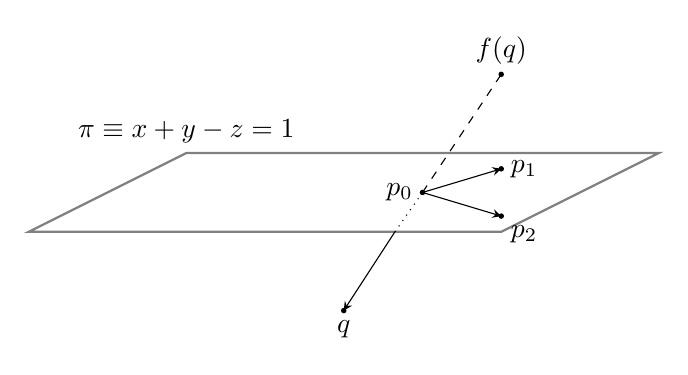
\begin{tikzpicture}
            % Definir los vértices del romboide
            \coordinate (A) at (0,0);
            \coordinate (B) at (2,1);
            \coordinate (C) at (8,1);
            \coordinate (D) at  (6,0);
        
            \coordinate (f_Q) at  (6,2);
            \coordinate (Q) at  (4,-1);
        
            \coordinate (p_0) at  (5,0.5);
            \coordinate (p_1) at  (6,0.8);
            \coordinate (p_2) at  (6,0.2);
        
            % Dibujar el romboide
            \draw[gray, thick] (A) -- (B) -- (C) -- (D) -- cycle;
            \node[above] at (B) {$\pi\equiv x+y-z=1$};
            
            % Dibujar el punto arriba
            \fill (Q) circle (1pt);
            \node[below] at (Q) {$q$};
            
            % Dibujar el punto abajo
            \fill (f_Q) circle (1pt);
            \node[above] at (f_Q) {$f(q)$};
            
            % Dibujar el punto en el plano
            \fill (p_0) circle (1pt);
            \node[left] at (p_0) {$p_0$};
        
            % Dibujar el punto en el plano
            \fill (p_1) circle (1pt);
            \node[right] at (p_1) {$p_1$};
        
            % Dibujar el punto en el plano
            \fill (p_2) circle (1pt);
            \node[below right] at (p_2) {$p_2$};
        
            \draw[dashed] (p_0) -- (f_Q);
            \draw[dotted] (4.65,0) -- (p_0);
            
            \draw[-stealth] (4.65, 0) -- (Q);
            \draw[-stealth] (p_0) -- (p_1);
            \draw[-stealth] (p_0) -- (p_2);
        \end{tikzpicture}
    \end{figure}
    
    Tenemos que $\vec{\pi}\equiv x+y-z=0$. Tomemos como los dos primeros vectores del sistema de referencia dos vectores linealmente independientes del plano:
    $$v_1=(1,-1,0)\qquad v_2=(1,0,1)$$

    Para obtener una base, tenemos que nos falta un vector. Notemos $q=(0,0,0)$, y sea $p_0=\left(\frac{1}{2},\frac{1}{2},0\right)\in \pi$, y tenemos que $v_3=\vec{p_0q}=q-p_0=\left(-\frac{1}{2},-\frac{1}{2},0\right)$. Entonces, tomando el sistema de coordenadas $\cc{R}=\{p_0,p_1,p_2,q\}=\{p_0,\cc{B}=\{v_1,v_2,v_3\}\}$, se tiene que ${p_0}_{\cc{R}}=(0,0,0)$. Además, tenemos que:
    \begin{equation*}
        \vec{f}(v_i)=\vec{f}(\vec{p_0p_i}) = \vec{f(p_0)f(p_i)} \AstIg \vec{p_0p_i} = v_i \qquad \forall i=1,2
    \end{equation*}
    donde en $(\ast)$ he aplicado que $v_1,v_2\in \vec{\pi}$, por lo que $p_0,p_1,p_2\in \pi$. Además,
    \begin{equation*}
        \vec{f}(v_3) = \vec{f}(\vec{p_0q}) = \vec{f(p_0)f(q)} = \vec{p_0f(q)} = f(q) - p_0 = (1,1,0) - \left(\frac{1}{2},\frac{1}{2},0\right) = \left(\frac{1}{2},\frac{1}{2},0\right) = -v_3
    \end{equation*}

    Por tanto, tenemos que la matriz que describe $\vec{f}$ es:
    \begin{equation*}
        M(\vec{f},\cc{B},\cc{B}) = \left(\begin{array}{ccc}
        1 & 0 & 0\\
        0 & 1 & 0 \\
        0 & 0 & -1\\
    \end{array}\right)
    \end{equation*}

    Como $f(p_0)=p_0$, tenemos que $f(p_0)_{\cc{R}}=(0,0,0)$. Por tanto,    
    \begin{equation*}
        M(f,\cc{R},\cc{R}) = \left(\begin{array}{c|ccc}
        1 & 0 & 0 & 0 \\ \hline
        0 & 1 & 0 & 0\\
        0 & 0 & 1 & 0 \\
        0 & 0 & 0 & -1\\
    \end{array}\right)
    \end{equation*}\\

    Buscamos ahora expresarlo en el sistema de referencia canónico $\cc{R}_0$. Tenemos que $f(0,0,0)=(1,1,0)$. Buscamos ahora $M(\vec{f}, \cc{B}_u, \cc{B}_u)$. Esta es:
    \begin{equation*}\begin{split}
        M(\vec{f}, \cc{B}_u, \cc{B}_u) &= M(\cc{B}, \cc{B}_u)\cdot M(\vec{f}, \cc{B}, \cc{B})\cdot M(\cc{B}_u, \cc{B}) =\\&
        = \left(\begin{array}{ccc}
            1 & 1 & \nicefrac{-1}{2}\\
            -1 & 0 & \nicefrac{-1}{2} \\
            0 & 1 & 0\\
        \end{array}\right)
        \left(\begin{array}{ccc}
            1 & 0 & 0\\
            0 & 1 & 0 \\
            0 & 0 & -1\\
        \end{array}\right)
        \left(\begin{array}{ccc}
            1 & 1 & \nicefrac{-1}{2}\\
            -1 & 0 & \nicefrac{-1}{2} \\
            0 & 1 & 0\\
        \end{array}\right)^{-1} =\\&=
        \left(\begin{array}{ccc}
            0 & -1 & 1\\
            -1 & 0 & 1 \\
            0 & 0 & 1\\
        \end{array}\right)
    \end{split}\end{equation*}

    Por tanto,
    \begin{equation*}
        M(f,\cc{R}_0,\cc{R}_0) = \left(\begin{array}{c|ccc}
        1 & 0 & 0 & 0 \\ \hline
        1 & 0 & -1 & 1\\
        1 & -1 & 0 & 1\\
        0 & 0 & 0 & 1\\
    \end{array}\right)
    \end{equation*}
    
\end{ejemplo}



\subsection{Aplicaciones afines notables}

Estas son las traslaciones, homotecias, proyecciones y simetrías. Para clasificarlas, se emplea la noción de punto fijo, descrita a continuación.
\begin{definicion}[Punto fijo]
    Sea $\cc{A}$ un espacio afín, y consideramos $f:\cc{A}\to \cc{A}$ una aplicación afín. Decimos que $p\in \cc{A}$ es un punto fijo de $f$ si y solo si $f(p)=p$.

    También decimos que $f$ deja invariante a $p$.\\

    Denotamos por $\cc{P}_f$ al conjunto de puntos fijos de $f$:
    \begin{equation*}
        \cc{P}_f = \{p\in \cc{A}\mid f(p)=p\} \subset \cc{A}
    \end{equation*}
\end{definicion}

\subsubsection{Traslaciones}
Recordamos que están descritas en la Definición \ref{def:traslacion}. 

Veamos este teorema, que es la generalización de un resultado de gran utilidad que veremos más adelante.
\begin{teo}
    Sean $\cc{A},\cc{A}'$ espacios afines, y consideramos $f,g:\cc{A}\to \cc{A}'$ aplicaciones afines. Entonces:
    \begin{equation*}
        \exists v_0\in \vec{\cc{A'}}\mid f=t_{v_0}\circ g \Longleftrightarrow \vec{f}=\vec{g}
    \end{equation*}

    Además, en ese caso $v_0=\vec{g(p)f(p)}\in \vec{\cc{A}'}$ para todo $p\in \cc{A}$ (el vector $v$ no depende de $p\in \cc{A}$).
\end{teo}
\begin{proof}\
    \begin{description}
        \item[$\Longleftarrow)$] Sea $v_0=\vec{g(p)f(p)}~\forall p\in \cc{A}'$. Veamos que no depende del valor de $p$:
        \begin{multline*}
            \vec{g(p)f(p)} = \vec{g(p')f(p')} \Longleftrightarrow f(p)-g(p) = f(p')-g(p') \Longleftrightarrow \\ \Longleftrightarrow \vec{f(p')f(p)} = \vec{g(p')g(p)} \Longleftrightarrow \vec{f}(\vec{p'p}) = \vec{g}(\vec{p'p}) \stackrel{(\ast)}{\Longrightarrow} \vec{p'p} = \vec{p'p}
        \end{multline*}
        lo cual es cierto para todo $p,p'\in \cc{A}$. Además, en $(\ast)$ he aplicado que $\vec{f}=\vec{g}$. Por tanto, tenemos que $v_0\in \vec{\cc{A}'}$ no depende del valor de $p$ escogido.

        Veamos que $f=t_{v_0}\circ g$:
        \begin{equation*}
            (t_{v_0}\circ g)(p) = t_{v_0}(g(p)) = g(p) + v_0 = g(p) + \vec{g(p)f(p)} = f(p) \qquad \forall p\in \cc{A}
        \end{equation*}

        \item[$\Longrightarrow)$] Se tiene que:
        \begin{equation*}
            \vec{f} = \vec{t_{v_0}\circ g} = \vec{t_{v_0}}\circ \vec{g} = Id_{\vec{\cc{A}'}}\circ \vec{g} = \vec{g}
        \end{equation*}

        Veamos ahora el valor de $v_0$. Tenemos que $f(p)=t_{v_0}(g(p)) = g(p)+v_0$, por lo que $v_0=f(p)-g(p)=\vec{g(p)f(p)}$.
    \end{description}
\end{proof}

En el teorema anterior, tomando $g=Id_{\cc{A}}$, tenemos el siguiente resultado, que nos es de gran utilidad para caracterizar las traslaciones.
\begin{coro}
    Sea $\cc{A}$ un espacio afín, y $f:\cc{A}\to \cc{A}$ una aplicación. Entonces:
    \begin{equation*}
        \exists v_0\in \vec{\cc{A}}\mid f=t_{v_0} \Longleftrightarrow f\text{ es afín }\land \vec{f}=Id_{\vec{\cc{A}}} 
    \end{equation*}

    Además, en ese caso $v_0=\vec{pf(p)}\in \vec{\cc{A}}$ para todo $p\in \cc{A}$ (el vector $v$ no depende de $p\in \cc{A}$).
\end{coro}

Además, es importante notar que:
\begin{equation*}
    \cc{P}_{t_v}\neq \emptyset \Longleftrightarrow v=\vec{0}.
\end{equation*}

Un aspecto importante de las traslaciones es que llevan rectas en rectas paralelas. Esto se puede ver en la siguiente proposición.
\begin{prop}
    Sea $\cc{A}$ un espacio afín, y $f:\cc{A}\to \cc{A}$ una traslación afín según el vector $v_0\in \vec{\cc{A}}$. Entonces, $f$ lleva rectas en rectas paralelas. Es decir,
    \begin{equation*}
        f(R)\| R \qquad \forall R\subset \cc{A}
    \end{equation*}
\end{prop}
\begin{proof}
    Sea $R=p+\vec{R}\subset \cc{A}$ una recta. Entonces, como $\vec{f}=Id$, tenemos que:
    \begin{equation*}
        f(R) = f(p+\vec{R}) = f(p) + \vec{f}(\vec{R}) = p+v_0 + Id(\vec{R}) = p' + \vec{R}
    \end{equation*}
    Por tanto, $f(R)\| R$.
\end{proof}

Respecto a la composición de traslaciones, tenemos el siguiente resultado, de demostración inmediata.
\begin{prop}
    Sean $f,g:\cc{A}\to \cc{A}$ dos traslaciones afines según los vectores $v_0,v_1\in \vec{\cc{A}}$, respectivamente. Entonces, se tiene que:
    \begin{equation*}
        f\circ g = t_{v_0+v_1}
    \end{equation*}
\end{prop}
Como la suma en $\vec{\cc{A}}$ es conmutativa, tenemos que $f\circ g = g\circ f$.

\subsubsection{Homotecias afines}

\begin{definicion}[Homotecia afín]
    Sea $\cc{A}$ un espacio afín. Definimos la homotecia afín de centro $o\in \cc{A}$ y razón (o radio) $k\in\bb{R}$, como:
    \Func{H_{o,k}}{\cc{A}}{\cc{A}}{p}{o+k\cdot \vec{op}}
\end{definicion}
\begin{observacion}
    A menudo, se establece la condición de que $k\neq 0,1$, ya que son casos particulares. \begin{itemize}
        \item En el caso de $k=1$, tenemos que $H_{o,1}=Id_{\cc{A}}$.
        \item En el caso de $k=0$, tenemos que $H_{o,0}=o$ aplicación constante en $o$.
    \end{itemize}
\end{observacion}

El siguiente resultado se estudia para valores de $k\neq 0,1$, ya que como hemos visto, estos son casos particulares que ya conocemos.
\begin{prop}
    Sea $\cc{A}$ un espacio afín, y $f:\cc{A}\to \cc{A}$ una aplicación. Entonces, dado $k\in \bb{R}\setminus \{0,1\}$, tenemos:
    \begin{equation*}
        \exists o\in \cc{A}\mid f=H_{o,k} \Longleftrightarrow f\text{ es afín }\land \vec{f}=kId_{\vec{\cc{A}}} 
    \end{equation*}

    Además, el único punto fijo de $f$ es su centro $o\in \cc{A}$, que cumple que
    \begin{equation*}
        o = p+\frac{1}{1-k}\vec{pf(p)} \qquad \forall p\in \cc{A}
    \end{equation*}
\end{prop}
\begin{proof}\
    \begin{description}
        \item[$\Longrightarrow)$] En primer lugar, tenemos que:
        \begin{equation*}
            H_{o,k}(o)=o+k\vec{0} = o \qquad \forall k\in \bb{R}
        \end{equation*}
        
        Veamos cuál es su aplicación lineal asociada:
        \begin{equation*}
            \vec{H_{o,k}}\left(\vec{op}\right) = \vec{H_{o,k}(o)H_{o,k}(p)} = \vec{oH_{o,k}(p)} = o+k\vec{op} -o = k\vec{op} = kI_{\vec{\cc{A}}}\left(\vec{op}\right)
        \end{equation*}
        
        Por tanto, tenemos que $H_{o,k}$ es una aplicación afín con aplicación afín asociada la identidad de razón $k$, $kI_{\vec{\cc{A}}}$.

        Veamos ahora que el centro cumple dicha expresión:
        \begin{equation*}
            p+\frac{1}{1-k}\vec{pf(p)} = p + \frac{1}{1-k}[f(p)-p]
            = p + \frac{1}{1-k}[o+k\vec{op}-p]
            = p + \frac{1}{1-k}[(1-k)(o-p)] = o
        \end{equation*}

        \item[$\Longleftarrow)$] Sea $o=p+\frac{1}{1-k}\cdot \vec{pf(p)}\in \cc{A}~~\forall p\in \cc{A}$.
        Veamos que $o$ no depende del valor de $p$ dado. 
        Sea $p'\in \cc{A}$. Entonces:
        \begin{multline*}
            p+\frac{1}{1-k}\cdot \vec{pf(p)} = p'+\frac{1}{1-k}\cdot \vec{p'f(p')} \Longleftrightarrow \\ \Longleftrightarrow
            p-p' = \frac{\vec{p'f(p')} - \vec{pf(p)}}{1-k}
            = \frac{f(p')-p'-f(p)+p}{1-k}
            = \frac{p-p' - \vec{f(p')f(p)}}{1-k}
            =\\\AstIg \frac{\vec{p'p} - \vec{f}(\vec{p'p})}{1-k} = \frac{\vec{p'p} - k\cdot \vec{p'p}}{1-k} = \vec{p'p} = p-p'
        \end{multline*}
        donde en $(\ast)$ he aplicado el valor de $\vec{f}$. Veamos que $f(o)=o$, es decir, que $o$ es un punto fijo de $f$:
        \begin{equation*}\begin{split}
            f(o)=&f(p)  +\frac{1}{1-k}\cdot \vec{f}(\vec{pf(p)})
            =f(p)  +\frac{1}{1-k}\cdot k\cdot \vec{pf(p)}
            =\frac{(1-k)f(p) + kf(p) - kp}{1-k} =\\
            =&\frac{f(p) - kp}{1-k}
            =\frac{f(p) - kp + p-p}{1-k}
            =\frac{f(p)-p + (1-k)p}{1-k} = p + \frac{1}{1-k}\vec{pf(p)} = o
        \end{split}\end{equation*}

        Veamos ahora que $f$ es una homotecia. Sea $p\in \cc{A}$. Tenemos que $p=o+\vec{op}$.
        \begin{equation*}
            f(p) = f(o)+\vec{f}(\vec{op}) = o+k\vec{op} = H_{o,k}(p) \qquad \forall p\in \cc{A}
        \end{equation*}

        Por tanto, tenemos que $\exists o\in \cc{A}$ tal que $f=H_{o,k}$.
    \end{description}\vspace{1cm}
    
    Veamos ahora que el único punto fijo es el centro:
    \begin{equation*}
        f(p)=p \Longleftrightarrow o+k\vec{op} = p \Longleftrightarrow o+kp-ko = p \Longleftrightarrow (1-k)o = (1-k)p \Longleftrightarrow p=o
    \end{equation*}
\end{proof}
Por tanto, hemos demostrado que una homotecia de razón $k\neq 0,1$ tan solo tiene un punto fijo, que es su centro.

\begin{definicion}[Simetría central]
    Dado un espacio afín $\cc{A}$, y un punto $o\in \cc{A}$, definimos la simetría central de centro $o$ como la homotecia de centro $o$ y razón $-1$, $H_{o,-1}$.
\end{definicion}

Para la siguiente caracterización, usaremos la definición de punto medio, dada en la Definición \ref{def:PuntoMedio}.
\begin{prop}
    Sea $\cc{A}$ un espacio afín, y $f:\cc{A}\to \cc{A}$ una aplicación. Entonces, equivalen:
    \begin{enumerate}
        \item $f$ es una simetría central.
        \item $f$ es afín y $\vec{f}=-Id_{\vec{\cc{A}}}$.
        \item $\exists o\in \cc{A}\mid m_{pf(p)}=o \qquad \forall p\in \cc{A}$.
    \end{enumerate}
\end{prop}
\begin{proof}
    La equivalencia entre $1)$ y $2)$ se ha demostrado ya, ya que una simetría central es una homotecia de razón $-1$.
    Veamos ahora la equivalencia entre $1)$ y $3)$. Como $m_{pf(p)}= o + \frac{1}{2}\left(\vec{op} + \vec{pf(p)}\right)$, tenemos que:
    \begin{multline*}
        \exists o\in \cc{A}\mid m_{pf(p)}=o ~~ \forall p\in \cc{A} \Longleftrightarrow \\ \Longleftrightarrow
        \exists o\in \cc{A}\mid \vec{op}+\vec{of(p)} = \vec{0} ~~ \forall p\in \cc{A} \Longleftrightarrow \\ \Longleftrightarrow
        \exists o\in \cc{A}\mid f(p) = o - \vec{op} ~~ p\in \cc{A} \Longleftrightarrow 
        f = H_{o,-1}
    \end{multline*}
\end{proof}

Al igual que con las traslaciones, las homotecias llevan rectas en rectas paralelas. Esto se puede ver en la siguiente proposición.
\begin{prop}
    Sea $\cc{A}$ un espacio afín, y $H_{o,k}:\cc{A}\to \cc{A}$ una homotecia afín de centro $o\in \cc{A}$ y razón $k\in \bb{R}$. Entonces, $H_{o,k}$ lleva rectas en rectas paralelas. Es decir,
    \begin{equation*}
        H_{o,k}(R)\| R \qquad \forall R\subset \cc{A}
    \end{equation*}
\end{prop}
\begin{proof}
    Sea $R=p+\vec{R}\subset \cc{A}$ una recta. Entonces, como $\vec{f}=k~Id$, tenemos que:
    \begin{equation*}
        f(R) = f(p+\vec{R}) = f(p) + \vec{f}(\vec{R}) = f(p) + k~Id(\vec{R}) \AstIg f(p) + \vec{R}
    \end{equation*}
    donde en $(\ast)$ he aplicado que $\vec{R}$ es cerrado para producto por escalares. Por tanto, $f(R)\| R$.
\end{proof}

Respecto a la composición de homotecias, tenemos el siguiente resultado:
\begin{prop}
    Sean $f,g:\cc{A}\to \cc{A}$ dos homotecias afines de razones $k_1,k_2\in \bb{R}$, respectivamente y ambas de centro $o\in \cc{A}$. Entonces, se tiene que:
    \begin{equation*}
        f\circ g = H_{o,k_1\cdot k_2}
    \end{equation*}
\end{prop}
\begin{proof}
    Sea $p\in \cc{A}$. Entonces, tenemos que:
    \begin{multline*}
        f(g(p)) = f(o+k_2\vec{op}) = o+k_1\vec{o(g(p))} = o + k_1(g(p)-o) =\\= o + k_1(\cancel{o}+k_2\vec{op}-\cancel{o}) = o + k_1k_2\vec{op} = H_{o,k_1k_2}(p) \qedhere
    \end{multline*}
\end{proof}
Notemos que, como la multiplicación de números reales es conmutativa, tenemos que $f\circ g = g\circ f$.


\begin{definicion}
    Una aplicación afín se dice que es una dilatación si y solo si es una homotecia o una traslación.
\end{definicion}

\subsubsection{Proyecciones y Simetrías}
\begin{notacion}
    Antes de presentar las proyecciones y las simetrías en el espacio afín, recordamos cómo las notamos en el caso de espacios vectoriales.
    
    Sea $\vec{V}$ un espacio vectorial, y consideramos $\vec{U},\vec{W}\subset\vec{V}$ subespacios vectoriales de $\vec{V}$ tal que $\vec{V}=\vec{U}\oplus \vec{W}$. La proyección sobre $\vec{U}$ se nota por $\pi_{\vec{U}}$, mientras que la simetría sobre $\vec{U}$ se nota por $\sigma_{\vec{U}}$.
\end{notacion}
\begin{definicion}[Proyección]
    Sea $\cc{A}$ un espacio afín, y sean $S,T$ subespacios afines complementarios de $\cc{A}$. Entonces, por la Proposición \ref{prop:ComplementariosSumaIntersec}, tenemos que $S\cap T=\{p_0\}$. Entonces, definimos la proyección afín en $S$ paralela a $T$ como:
    \Func{\pi_{S,T}}{\cc{A}}{S}{q}{p_0+\pi_{\vec{S}, \vec{T}}\left(\vec{p_0q}\right)}
\end{definicion}
\begin{figure}[H]
    \centering
    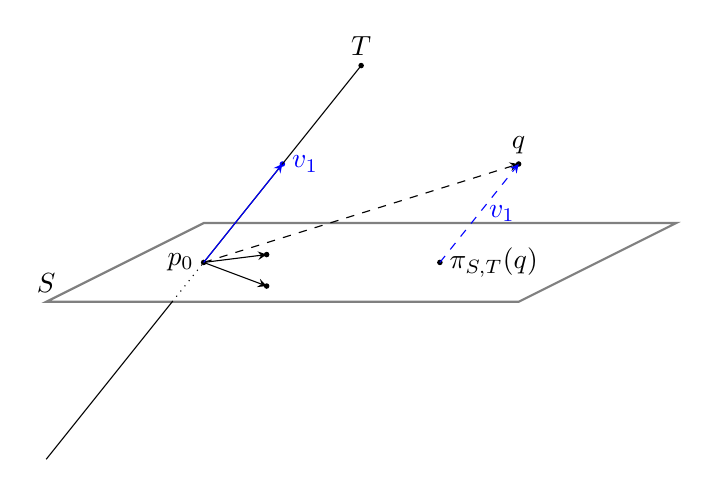
\begin{tikzpicture}
        % Definir los vértices del romboide
        \coordinate (A) at (0,0);
        \coordinate (B) at (2,1);
        \coordinate (C) at (8,1);
        \coordinate (D) at  (6,0);
    
        \coordinate (T_arr) at  (4,3);
        \coordinate (T_ab) at  (0,-2);

        \coordinate (Q) at  (6,1.75);
        \coordinate (pro) at  (5,0.5);
        
        \coordinate (p_0) at  (2,0.5);
        \coordinate (p_1) at  (2.8,0.6);
        \coordinate (p_2) at  (2.8,0.2);
        \coordinate (p_3) at  (3, 1.75);
    
        % Dibujar el romboide
        \draw[gray, thick] (A) -- (B) -- (C) -- (D) -- cycle;
        \node[above] at (A) {$S$};
            
        % Dibujar el punto arriba
        \fill (Q) circle (1pt);
        \node[above] at (Q) {$q$};

        % Dibujar la proyección
        \fill (pro) circle (1pt);
        \node[right] at (pro) {$\pi_{S,T}(q)$};

        \draw[dashed, -stealth] (p_0) -- (Q);
        \draw[dashed, -stealth, blue] (pro) -- node[right]{$v_1$} (Q);
        
        % Dibujar el punto arriba
        \fill (T_arr) circle (1pt);
        \node[above] at (T_arr) {$T$};
        
        % Dibujar el punto en el plano
        \fill (p_0) circle (1pt);
        \node[left] at (p_0) {$p_0$};
    
        % Dibujar el punto en el plano
        \fill (p_1) circle (1pt);
    
        % Dibujar el punto en el plano
        \fill (p_2) circle (1pt);

        % Dibujar el punto en el plano
        \fill[blue] (p_3) circle (1pt);
        \node[right, blue] at (p_3) {$v_1$};
    
        \draw (p_0) -- (T_arr);
        \draw[dotted] (1.6,0) -- (p_0);
        
        \draw (1.6, 0) -- (T_ab);
        \draw[-stealth] (p_0) -- (p_1);
        \draw[-stealth] (p_0) -- (p_2);
        \draw[-stealth, blue] (p_0) -- (p_3);
    \end{tikzpicture}
    \caption{Representación gráfica de la proyección afín.}
\end{figure}    

Respecto a las proyecciones, tenemos los siguientes resultados:
\begin{prop}
    Sea $\cc{A}$ un espacio afín, y sean $S,T$ subespacios afines complementarios de $\cc{A}$. Entonces:
    \begin{enumerate}
        \item $\pi_{S,T}:\cc{A}\to S$ es una aplicación afín, con $\vec{\pi_{S,T}}=\pi_{\vec{S}, \vec{T}}$.
        \item $\cc{P}_{\pi_{S,T}}=Im(\pi_{S,T})=S$.
        \item $\pi_{S,T}\circ \pi_{S,T} =\pi_{S,T}$ (idempotencia).
        \item $\vec{q\pi_{S,T}(q)}\in \vec{T} \qquad \forall q\in \cc{A}$.
    \end{enumerate}
\end{prop}
\begin{proof} Demostramos cada resultado por separado:
\begin{enumerate}
    \item Veamos que la dada es la aplicación lineal asociada:
    \begin{multline*}
        \vec{\pi_{S,T}}(\vec{pq}) = \vec{\pi_{S,T}(p)\pi_{S,T}(q)} = \vec{(p_0+\pi_{\vec{S}, \vec{T}}(\vec{p_0p}))(p_0+\pi_{\vec{S}, \vec{T}}(\vec{p_0q}))} =\\= \pi_{\vec{S}, \vec{T}}(\vec{p_0q})-\pi_{\vec{S}, \vec{T}}(\vec{p_0p}) = \pi_{\vec{S}, \vec{T}}(\vec{pq})
    \end{multline*}
    donde he empleado que las proyecciones vectoriales son aplicaciones lineales.

    \item Veamos los puntos fijos de las proyecciones:
    \begin{equation*}
        \pi_{S,T}(q)=q \Longleftrightarrow p_0 + \pi_{\vec{S}, \vec{T}}(\vec{p_0q}) = q
        \Longleftrightarrow \pi_{\vec{S}, \vec{T}}(\vec{p_0q}) = \vec{p_0q}
        \Longleftrightarrow \vec{p_0q}\in \vec{S}
        \Longleftrightarrow q\in S
    \end{equation*}
    donde he aplicado que los vectores propios de $\pi_{\vec{S}, \vec{T}}$ con valor propio $1$ son los vectores de $\vec{S}$.

    \item Tenemos que $\pi_{S,T}(q)\in S$ para todo $q\in \cc{A}$. Por tanto, es un punto fijo, por lo que:
    \begin{equation*}
        (\pi_{S,T}\circ \pi_{S,T})(q) = \pi_{S,T}(\pi_{S,T}(q)) = \pi_{S,T}(q) \hspace{1cm} \forall q\in \cc{A}
    \end{equation*}

    \item Tenemos que:
    \begin{equation*}
        \vec{q\pi_{S,T}(q)} = \vec{q(p_0+\pi_{\vec{S}, \vec{T}}(\vec{p_0q}))}
        =  \vec{qp_0} + \pi_{\vec{S}, \vec{T}}(\vec{p_0q})
        =  -\vec{p_0q} + \pi_{\vec{S}, \vec{T}}(\vec{p_0q})
    \end{equation*}

    Como sabemos que $\vec{p_0q} = \pi_{\vec{S}, \vec{T}}(\vec{p_0q}) + \pi_{\vec{T}, \vec{S}}(\vec{p_0q})$, tenemos que
    \begin{equation*}
        \vec{q\pi_{S,T}(q)} = -\pi_{\vec{T}, \vec{S}}(\vec{p_0q}) \in \vec{T}
    \end{equation*}
\end{enumerate}
\end{proof}

\begin{definicion}[Simetría afín]
    Sea $\cc{A}$ un espacio afín, y sean $S,T$ subespacios afines complementarios de $\cc{A}$. Entonces, por la Proposición \ref{prop:ComplementariosSumaIntersec}, tenemos que $S\cap T=\{p_0\}$. Entonces, definimos la simetría (o reflexión) afín en $S$ paralela a $T$ como:
    \Func{\sigma_{S,T}}{\cc{A}}{\cc{A}}{q}{p_0+\sigma_{\vec{S}, \vec{T}}\left(\vec{p_0q}\right) = p_0+\pi_{\vec{S}, \vec{T}}\left(\vec{p_0q}\right)-\pi_{\vec{T}, \vec{S}}\left(\vec{p_0q}\right)}
\end{definicion}
\begin{figure}[H]
    \centering
    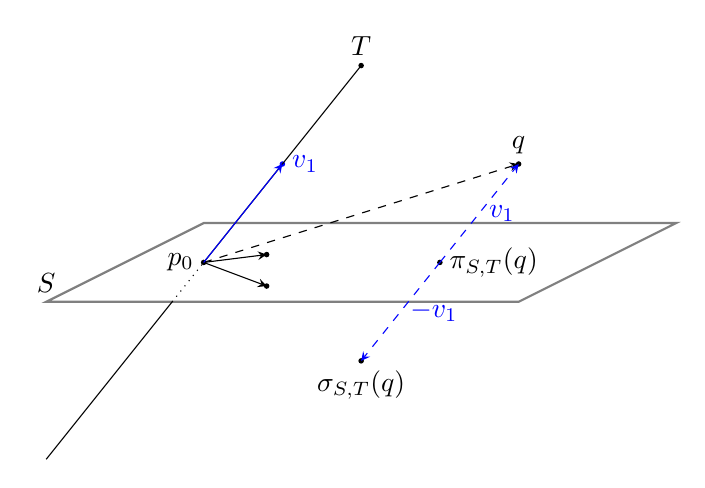
\begin{tikzpicture}
        % Definir los vértices del romboide
        \coordinate (A) at (0,0);
        \coordinate (B) at (2,1);
        \coordinate (C) at (8,1);
        \coordinate (D) at  (6,0);
    
        \coordinate (T_arr) at  (4,3);
        \coordinate (T_ab) at  (0,-2);

        \coordinate (Q) at  (6,1.75);
        \coordinate (pro) at  (5,0.5);
        \coordinate (ref) at  (4,-0.75);
        
        \coordinate (p_0) at  (2,0.5);
        \coordinate (p_1) at  (2.8,0.6);
        \coordinate (p_2) at  (2.8,0.2);
        \coordinate (p_3) at  (3, 1.75);
    
        % Dibujar el romboide
        \draw[gray, thick] (A) -- (B) -- (C) -- (D) -- cycle;
        \node[above] at (A) {$S$};
            
        % Dibujar el punto arriba
        \fill (Q) circle (1pt);
        \node[above] at (Q) {$q$};

        % Dibujar la proyección
        \fill (pro) circle (1pt);
        \node[right] at (pro) {$\pi_{S,T}(q)$};

        % Dibujar la proyección
        \fill (ref) circle (1pt);
        \node[below] at (ref) {$\sigma_{S,T}(q)$};

        \draw[dashed, -stealth] (p_0) -- (Q);
        \draw[dashed, -stealth, blue] (pro) -- node[right]{$v_1$} (Q);
        \draw[dashed, -stealth, blue] (pro) -- node[right]{$-v_1$} (ref);
        
        % Dibujar el punto arriba
        \fill (T_arr) circle (1pt);
        \node[above] at (T_arr) {$T$};
        
        % Dibujar el punto en el plano
        \fill (p_0) circle (1pt);
        \node[left] at (p_0) {$p_0$};
    
        % Dibujar el punto en el plano
        \fill (p_1) circle (1pt);
    
        % Dibujar el punto en el plano
        \fill (p_2) circle (1pt);

        % Dibujar el punto en el plano
        \fill[blue] (p_3) circle (1pt);
        \node[right, blue] at (p_3) {$v_1$};
    
        \draw (p_0) -- (T_arr);
        \draw[dotted] (1.6,0) -- (p_0);
        
        \draw (1.6, 0) -- (T_ab);
        \draw[-stealth] (p_0) -- (p_1);
        \draw[-stealth] (p_0) -- (p_2);
        \draw[-stealth, blue] (p_0) -- (p_3);
    \end{tikzpicture}
    \caption{Representación gráfica de la simetría afín.}
\end{figure}

Respecto a las simetrías, tenemos el primer resultado, de gran importancia a la hora de los ejercicios prácticos.
\begin{prop}
    Sea $\cc{A}$ un espacio afín, y sean $S,T$ subespacios afines complementarios de $\cc{A}$. Entonces:
    \begin{equation*}
        m_{p~\sigma_{S,T}(p)} = \pi_{S,T}(p) \qquad \forall p\in \cc{A}
    \end{equation*}
    En particular, $m_{p~\sigma_{S,T}(p)}\in S$ para todo $p\in \cc{A}$.
\end{prop}
\begin{proof}
    Sea $\{p_0\}=S\cap T$. Entonces, para todo $p\in \cc{A}$, tenemos que:
    \begin{align*}
        m_{p~\sigma_{S,T}(p)}
        &= p_0 + \frac{1}{2}\left(\vec{p_0p} + \vec{p_0\sigma_{S,T}(p)}\right)
        = p_0 + \frac{1}{2}\left(\vec{p_0p} -\cancel{p_0} + \cancel{p_0} + \sigma_{\vec{S},\vec{T}}(p_0p)\right)
        \AstIg \\ &\AstIg
        p_0 + \frac{1}{2}\left(\vec{p_0p} + 2\pi_{\vec{S},\vec{T}}(p_0p) - \vec{p_0p}\right)
        = p_0 + \pi_{\vec{S},\vec{T}}(p_0p) = \pi_{S,T}(p)
    \end{align*}
    donde en $(\ast)$ he aplicado que $\sigma_{\vec{S},\vec{T}}(p_0p) = 2\pi_{\vec{S},\vec{T}}(p_0p) - \vec{p_0p}$, como se demostró en Geometría II.

    En concreto, como $Im(\pi_{S,T})=S$, tenemos $m_{p~\sigma_{S,T}(p)}\in S$ para todo $p\in \cc{A}$.
\end{proof}

Además, tenemos los siguientes resultados:
\begin{prop}
    Sea $\cc{A}$ un espacio afín, y sean $S,T$ subespacios afines complementarios de $\cc{A}$. Entonces:
    \begin{enumerate}
        \item $\sigma_{S,T}:\cc{A}\to \cc{A}$ es una aplicación afín, con $\vec{\sigma_{S,T}}=\sigma_{\vec{S}, \vec{T}}$.
        \item $\cc{P}_{\sigma_{S,T}}=S$.
        \item $\sigma_{S,T}\circ \sigma_{S,T} =Id_{\cc{A}}$ (involución).
    \end{enumerate}
\end{prop}
\begin{proof} Demostramos cada resultado por separado:
\begin{enumerate}
    \item Veamos que la dada es la aplicación lineal asociada:
    \begin{multline*}
        \vec{\sigma_{S,T}}(\vec{pq}) = \vec{\sigma_{S,T}(p)\sigma_{S,T}(q)} = \vec{(p_0+\sigma_{\vec{S}, \vec{T}}(\vec{p_0p}))(p_0+\sigma_{\vec{S}, \vec{T}}(\vec{p_0q}))} =\\= \sigma_{\vec{S}, \vec{T}}(\vec{p_0q})-\sigma_{\vec{S}, \vec{T}}(\vec{p_0p}) = \sigma_{\vec{S}, \vec{T}}(\vec{pq})
    \end{multline*}
    donde he empleado que las simetrías vectoriales son aplicaciones lineales.

    \item Veamos los puntos fijos de las simetrías:
    \begin{equation*}
        \sigma_{S,T}(q)=q \Longleftrightarrow p_0 + \sigma_{\vec{S}, \vec{T}}(\vec{p_0q}) = q
        \Longleftrightarrow \sigma_{\vec{S}, \vec{T}}(\vec{p_0q}) = \vec{p_0q}
        \Longleftrightarrow \vec{p_0q}\in \vec{S}
        \Longleftrightarrow q\in S
    \end{equation*}
    donde he aplicado que los vectores propios de $\sigma_{\vec{S}, \vec{T}}$ con valor propio $1$ son los vectores de $\vec{S}$.

    \item En primer lugar, tenemos que $\vec{\sigma_{S,T}\circ \sigma_{S,T}} = \sigma_{\vec{S}, \vec{T}}\circ \sigma_{\vec{S}, \vec{T}} = Id_{\vec{A}}$.

    Además, $\exists a\in \cc{A}$ tal que $\sigma_{S,T}(a)=Id_{\cc{A}}(a)=a$, ya que $\sigma_{S,T}$ tiene puntos fijos.

    Por tanto, por el Teorema \ref{teo:UnicidadLinealAsociada}, se tiene.
\end{enumerate}
\end{proof}

Respecto a las simetrías, hay un caso particular, que es el de las simetrías respecto de un punto. En este caso, tenemos el siguiente resultado:
\begin{prop}\label{lema:SimetriaCentral}
    Sea $\cc{A}$ un espacio afín, y sea $o\in \cc{A}$ un punto. Entonces, se tiene:
    \begin{equation*}
        \sigma_{o} = H_{o,-1}
    \end{equation*}
    Es decir, la simetría respecto de un punto es una simetría central respecto de dicho punto.
\end{prop}
\begin{proof}
    Tenemos que $\sigma_{o}(o) = o$. Además, como $\vec{\{o\}} = \left\{\vec{0}\right\}$, tenemos que $\vec{\{o\}}^\perp=\cc{A}$. Por tanto,
    $\sigma_{\vec{\{o\}}}=-Id_{\vec{A}}$. Por el Teorema \ref{teo:UnicidadLinealAsociada}, tenemos que $\sigma_{o} = H_{o,-1}$.
\end{proof}




\section{Teoremas de Pappus y Desargues Afines}\label{sec:TeoremasPappusDesarguesAfines}
En esta sección, veremos dos teoremas que nos serán de gran utilidad para resolver ejercicios prácticos. Estos son el Teorema de Pappus y el Teorema de Desargues.

\begin{notacion}
    Sea $\cc{A}$ un espacio afín, y sean $p,q\in \cc{A}$ dos puntos distintos. Entonces, se denota la recta que pasa por $p,q$ como:
    \begin{equation*}
        R_{pq} = \{p+t\vec{pq}\mid t\in \bb{R}\}
    \end{equation*}
\end{notacion}
\begin{teo}[(afín) de Pappus]
    Sea $\cc{A}$ un plano afín, y sean $R_1, R_2$ dos rectas afines distintas de $\cc{A}$.
    Consideramos $a_1,b_1,c_1\in R_1\setminus R_1\cap R_2$, y $a_2,b_2,c_2\in R_2\setminus R_1\cap R_2$. Entonces:
    \begin{equation*}
        \left.
            \begin{array}{c}
                R_{a_1b_2} \| R_{a_2b_1} \\ \land \\ R_{b_1c_2} \| R_{b_2c_1}
            \end{array} 
        \right\} \Longrightarrow R_{a_1c_2} \| R_{a_2c_1}
    \end{equation*}
\end{teo}
\begin{proof}
    Distinguimos entre si las rectas son paralelas o no:
    \begin{enumerate}
        \item Rectas secantes, $R_1\not \| R_2$:
        \begin{figure}[H]
            \centering
            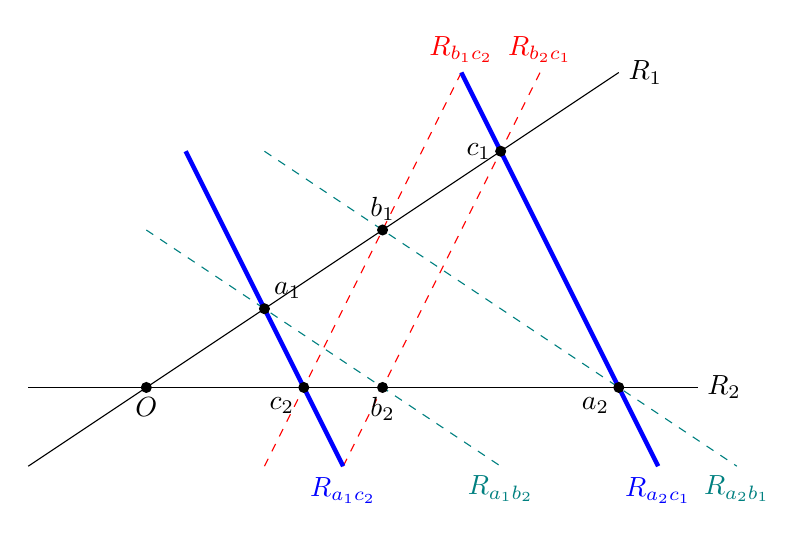
\begin{tikzpicture}
                \coordinate (a_1) at (1.5,1);
                \coordinate (b_1) at (3,2);
                \coordinate (c_1) at (4.5,3);

                \coordinate (a_2) at (6,0);
                \coordinate (b_2) at (3,0);
                \coordinate (c_2) at (2,0);

                \coordinate (R1_ini) at (-1.5,-1);
                \coordinate (R1_fin) at (6,4);

                \coordinate (R2_ini) at (-1.5,0);
                \coordinate (R2_fin) at (7,0);

                \coordinate (Ra1b2_ini) at (0,2);
                \coordinate (Ra1b2_fin) at (4.5,-1);

                \coordinate (Ra2b1_ini) at (1.5,3);
                \coordinate (Ra2b1_fin) at (7.5,-1);

                \coordinate (Rb1c2_ini) at (4,4);
                \coordinate (Rb1c2_fin) at (1.5,-1);

                \coordinate (Rb2c1_ini) at (5,4);
                \coordinate (Rb2c1_fin) at (2.5,-1);

                \coordinate (Ra1c2_ini) at (0.5,3);
                \coordinate (Ra1c2_fin) at (2.5,-1);

                \coordinate (Ra2c1_ini) at (4,4);
                \coordinate (Ra2c1_fin) at (6.5,-1);

                % Dibujamos R1 y R2
                \draw (R1_ini) -- (R1_fin) node [right] {$R_1$};
                \draw (R2_ini) -- (R2_fin) node [right] {$R_2$};

                % Dibujamos las rectas
                \draw[dashed, teal] (Ra1b2_ini) -- (Ra1b2_fin) node [below] {$R_{a_1b_2}$};
                \draw[dashed, teal] (Ra2b1_ini) -- (Ra2b1_fin) node [below] {$R_{a_2b_1}$};

                \draw[dashed, red] (Rb1c2_fin) -- (Rb1c2_ini) node [above] {$R_{b_1c_2}$};
                \draw[dashed, red] (Rb2c1_fin) -- (Rb2c1_ini) node [above] {$R_{b_2c_1}$};

                \draw[ultra thick, blue] (Ra1c2_ini) -- (Ra1c2_fin) node [below] {$R_{a_1c_2}$};
                \draw[ultra thick, blue] (Ra2c1_ini) -- (Ra2c1_fin) node [below] {$R_{a_2c_1}$};

                % Marcamos los puntos en R1 y R2
                \fill (a_1) circle (2pt) node [above right] {$a_1$};  
                \fill (b_1) circle (2pt) node [above] {$b_1$};
                \fill (c_1) circle (2pt) node [left] {$c_1$};

                \fill (a_2) circle (2pt) node [below left] {$a_2$};
                \fill (b_2) circle (2pt) node [below] {$b_2$};
                \fill (c_2) circle (2pt) node [below left] {$c_2$};

                % Marcamos el origen
                \coordinate (O) at (0,0);
                \fill (O) circle (2pt) node [below] {$O$};
            \end{tikzpicture}
            \caption{Representación gráfica del Teorema de Pappus para $R_1\not\|R_2$.}
        \end{figure}
        
        Sea $\{O\}=R_1\cap R_2$. Consideramos la homotecia $h_1$ de centro $O$ y que lleva $a_1\mapsto b_1$.
        Consideramos también la homotecia $h_2$ de centro $O$ y que lleva $b_1\mapsto c_1$.

        Como una traslación lleva rectas en rectas paralelas, tenemos que:
        \begin{equation*}
            \left\{
                \begin{array}{c}
                    R_{a_1b_2} \| R_{a_2b_1} \\
                    \land \\
                    h_1(a_1) = b_1
                \end{array}
            \right\} \Longrightarrow h_1(b_2)=a_2
            \hspace{1cm}
            \left\{
                \begin{array}{c}
                    R_{b_1c_2} \| R_{b_2c_1} \\
                    \land \\
                    h_2(b_1) = c_1
                \end{array}
            \right\} \Longrightarrow h_2(c_2)=b_2
        \end{equation*}

        Por tanto, tenemos que:
        \begin{figure}[H]
            \centering
            \shorthandoff{"}
            \begin{tikzcd}[column sep=large]
                % De a_1 a b_1 por h_1, y de b_1 a c_1 por h_2
                a_1 \arrow[r,maps to, "h_1"] & b_1 \arrow[r,maps to, "h_2"] & c_1 \\
                % De c_2 a b_2 por h_2, y de b_2 a a_2 por h_1
                c_2 \arrow[r,maps to, "h_2"] & b_2 \arrow[r,maps to, "h_1"] & a_2
            \end{tikzcd}
            \shorthandon{"}
        \end{figure}
        Es decir, $(h_2\circ h_1)(a_1)=c_1$ y $(h_1\circ h_2)(c_2)=a_2$. Como $h_2\circ h_1=h_1\circ h_2$, sea $h$ dicha homotecia de centro $O$. Entonces, tenemos que:
        \begin{equation*}
            \begin{split}
                \vec{h}(\vec{a_1c_2}) &= \vec{h(a_1)h(c_2)} = \vec{c_1a_2} \\
                &= k\cdot \vec{a_1c_2}
            \end{split} 
        \end{equation*}
        Por tanto, tenemos que $\vec{R_{a_1c_2}} = \cc{L}\{\vec{a_1c_2}\} = \cc{L}\{k\cdot \vec{a_1c_2}\} = \cc{L}\{\vec{c_1a_2}\} = \vec{R_{c_1a_2}}$. Por tanto, $R_{a_1c_2}\| R_{c_1a_2}$.







        
        \item Rectas paralelas, $R_1\| R_2$:
        \begin{figure}[H]
            \centering
            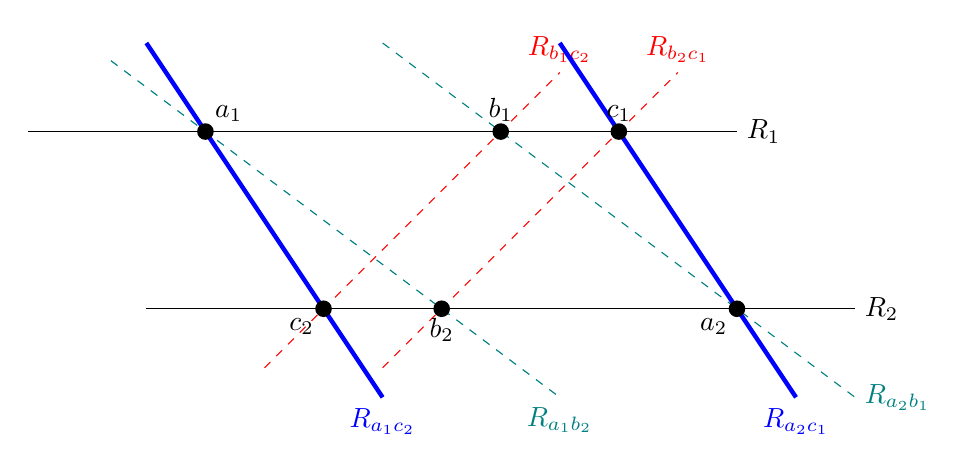
\begin{tikzpicture}[scale=1.5]
                \coordinate (a_1) at (1.5,1.5);
                \coordinate (b_1) at (4,1.5);
                \coordinate (c_1) at (5,1.5);

                \coordinate (a_2) at (6,0);
                \coordinate (b_2) at (3.5,0);
                \coordinate (c_2) at (2.5,0);

                \coordinate (R1_ini) at (0,1.5);
                \coordinate (R1_fin) at (6,1.5);

                \coordinate (R2_ini) at (1,0);
                \coordinate (R2_fin) at (7,0);

                \coordinate (Ra1b2_ini) at (0.7,2.1);
                \coordinate (Ra1b2_fin) at (4.5,-0.75);

                \coordinate (Ra2b1_ini) at (3,2.25);
                \coordinate (Ra2b1_fin) at (7,-0.75);

                \coordinate (Rb1c2_ini) at (2,-0.5);
                \coordinate (Rb1c2_fin) at (4.5,2);

                \coordinate (Rb2c1_ini) at (3,-0.5);
                \coordinate (Rb2c1_fin) at (5.5,2);

                \coordinate (Ra1c2_ini) at (1,2.25);
                \coordinate (Ra1c2_fin) at (3,-0.75);

                \coordinate (Ra2c1_ini) at (6.5, -0.75);
                \coordinate (Ra2c1_fin) at (4.5,2.25);

                % Dibujamos R1 y R2
                \draw (R1_ini) -- (R1_fin) node [right] {$R_1$};
                \draw (R2_ini) -- (R2_fin) node [right] {$R_2$};

                % Dibujamos las rectas
                \draw[dashed, teal] (Ra1b2_ini) -- (Ra1b2_fin) node [below] {$R_{a_1b_2}$};
                \draw[dashed, teal] (Ra2b1_ini) -- (Ra2b1_fin) node [right] {$R_{a_2b_1}$};

                \draw[dashed, red] (Rb1c2_ini) -- (Rb1c2_fin) node [above] {$R_{b_1c_2}$};
                \draw[dashed, red] (Rb2c1_ini) -- (Rb2c1_fin) node [above] {$R_{b_2c_1}$};

                \draw[ultra thick, blue] (Ra1c2_ini) -- (Ra1c2_fin) node [below] {$R_{a_1c_2}$};
                \draw[ultra thick, blue] (Ra2c1_fin) -- (Ra2c1_ini) node [below] {$R_{a_2c_1}$};

                % Marcamos los puntos en R1 y R2
                \fill (a_1) circle (2pt) node [above right] {$a_1$};  
                \fill (b_1) circle (2pt) node [above] {$b_1$};
                \fill (c_1) circle (2pt) node [above] {$c_1$};

                \fill (a_2) circle (2pt) node [below left] {$a_2$};
                \fill (b_2) circle (2pt) node [below] {$b_2$};
                \fill (c_2) circle (2pt) node [below left] {$c_2$};
            \end{tikzpicture}
            \caption{Representación gráfica del Teorema de Pappus para $R_1\|R_2$.}
        \end{figure}
        
        Consideramos la traslación $t_1$ según el vector $\vec{a_1 b_1}$ y la traslación $t_2$ según el vector $\vec{b_1 c_1}$.
        Notemos que, como $R_1\|R_2$, ambas rectas quedan fijas por $t_1$ y $t_2$.

        Como una homotecia lleva rectas en rectas paralelas, tenemos que:
        \begin{equation*}
            \left\{
                \begin{array}{c}
                    R_{a_1b_2} \| R_{a_2b_1} \\
                    \land \\
                    t_1(a_1) = b_1
                \end{array}
            \right\} \Longrightarrow t_1(b_2)=a_2
            \hspace{1cm}
            \left\{
                \begin{array}{c}
                    R_{b_1c_2} \| R_{b_2c_1} \\
                    \land \\
                    t_2(b_1) = c_1
                \end{array}
            \right\} \Longrightarrow t_2(c_2)=b_2
        \end{equation*}

        Por tanto, tenemos que:
        \begin{figure}[H]
            \centering
            \shorthandoff{"}
            \begin{tikzcd}[column sep=large]
                % De a_1 a b_1 por t_1, y de b_1 a c_1 por t_2
                a_1 \arrow[r,maps to, "t_1"] & b_1 \arrow[r,maps to, "t_2"] & c_1 \\
                % De c_2 a b_2 por t_2, y de b_2 a a_2 por t_1
                c_2 \arrow[r,maps to, "t_2"] & b_2 \arrow[r,maps to, "t_1"] & a_2
            \end{tikzcd}
            \shorthandon{"}
        \end{figure}
        Es decir, $(t_2\circ t_1)(a_1)=c_1$ y $(t_1\circ t_2)(c_2)=a_2$. Como $t_2\circ t_1=t_1\circ t_2$, sea $t$ dicha traslación según el vector $\vec{a_1b_1}+\vec{b_1c_1}=\vec{a_1c_1}$. Entonces, tenemos que:
        \begin{equation*}
            \begin{split}
                \vec{t}(\vec{a_1c_2}) &= \vec{t(a_1)t(c_2)} = \vec{c_1a_2} \\
                &= \vec{a_1c_2}
            \end{split} 
        \end{equation*}
        Por tanto, tenemos que $\vec{R_{a_1c_2}} = \cc{L}\{\vec{a_1c_2}\} = \cc{L}\{\vec{c_1a_2}\} = \vec{R_{c_1a_2}}$. Por tanto, $R_{a_1c_2}\| R_{c_1a_2}$.\qedhere
    \end{enumerate}
\end{proof}

Gráficamente, el Teorema de Pappus se puede ver en el siguiente applet de Geogebra: 
\href{https://www.geogebra.org/m/dd5s4mgc}{https://www.geogebra.org/m/dd5s4mgc}.

\begin{teo}[(afín) de Desargues]
    Sea $\cc{A}$ un espacio afín y sean $T_1=\{a_1,b_1,c_1\}$ $T_2=\{a_2,b_2,c_2\}$ dos triángulos de $\cc{A}$.
    Si los triángulos no tienen vértices comunes y sus lados son paralelos dos a dos
    (es decir, $R_{a_1b_1}\|R_{a_2b_2}$, $R_{a_1c_1}\|R_{a_2c_2}$ y $R_{b_1c_1}\|R_{b_2c_2}$), entonces
    las tres rectas $R_{a_1a_2}$, $R_{b_1b_2}$ y $R_{c_1c_2}$ son, o bien paralelas, o bien secantes en el mismo punto.

    \begin{figure}[H]
        \centering
        \begin{subfigure}{0.5\linewidth}
            \centering\hspace{-0.3cm}
            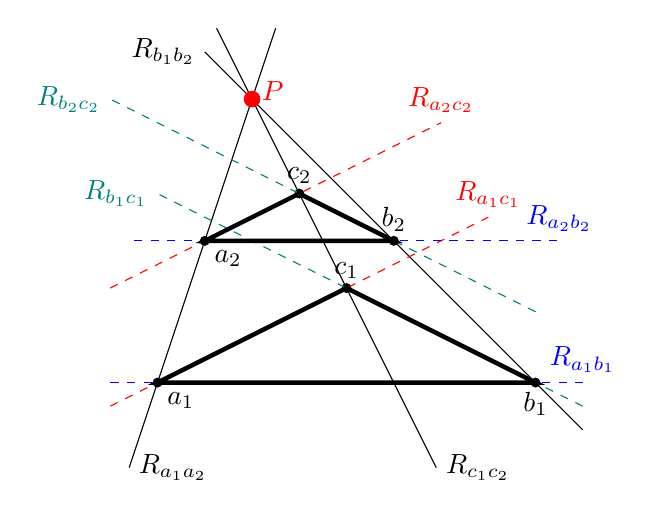
\begin{tikzpicture}[scale=0.6]
                % Los puntos del triángulo 1
                \coordinate (a_1) at (-4,0);
                \coordinate (b_1) at (4,0);
                \coordinate (c_1) at (0,2);

                % Los puntos del triángulo 2
                \coordinate (a_2) at (-3,3);
                \coordinate (b_2) at (1,3);
                \coordinate (c_2) at (-1,4);

                % Las rectas que unen los triángulos
                \coordinate (R_a1a2_ini) at (-4.6,-1.8);
                \coordinate (R_a1a2_fin) at (-1.5,7.5);

                \coordinate (R_c1c2_ini) at (1.9,-1.8);
                \coordinate (R_c1c2_fin) at (-2.75,7.5);

                \coordinate (R_b1b2_ini) at (5,-1);
                \coordinate (R_b1b2_fin) at (-3,7);

                % Las rectas que unen los vértices del triángulo 1
                \coordinate (R_a1b1_ini) at (-5,-0.5);
                \coordinate (R_a1b1_fin) at (3,3.5);

                \coordinate (R_a1c1_ini) at (-5,0);
                \coordinate (R_a1c1_fin) at (5,0);

                \coordinate (R_b1c1_ini) at (5,-0.5);
                \coordinate (R_b1c1_fin) at (-4,4);

                % Las rectas que unen los vértices del triángulo 2
                \coordinate (R_a2b2_ini) at (-5,2);
                \coordinate (R_a2b2_fin) at (2,5.5);

                \coordinate (R_a2c2_ini) at (-4.5,3);
                \coordinate (R_a2c2_fin) at (4.5,3);

                \coordinate (R_b2c2_ini) at (-5,6);
                \coordinate (R_b2c2_fin) at (4,1.5);

                % Punto de intersección de las rectas
                \coordinate (P) at (-2,6);

                % Dibujamos los puntos del triángulo 1
                \fill (a_1) circle (3pt) node [below right] {$a_1$};
                \fill (b_1) circle (3pt) node [below] {$b_1$};
                \fill (c_1) circle (3pt) node [above] {$c_1$};

                % Dibujamos los puntos del triángulo 2
                \fill (a_2) circle (3pt) node [below right] {$a_2$};
                \fill (b_2) circle (3pt) node [above] {$b_2$};
                \fill (c_2) circle (3pt) node [above] {$c_2$};

                % Dibujamos las rectas que unen los triángulos
                \draw[] (R_a1a2_fin) -- (R_a1a2_ini) node [right] {$R_{a_1a_2}$};
                \draw[] (R_b1b2_ini) -- (R_b1b2_fin) node [left] {$R_{b_1b_2}$};
                \draw[] (R_c1c2_fin) -- (R_c1c2_ini) node [right] {$R_{c_1c_2}$};

                % Dibujamos las rectas que unen los vértices del triángulo 1
                \draw[dashed, red] (R_a1b1_ini) -- (R_a1b1_fin) node [above] {$R_{a_1c_1}$};
                \draw[dashed, blue] (R_a1c1_ini) -- (R_a1c1_fin) node [above] {$R_{a_1b_1}$};
                \draw[dashed, teal] (R_b1c1_ini) -- (R_b1c1_fin) node [left] {$R_{b_1c_1}$};

                % Dibujamos las rectas que unen los vértices del triángulo 2
                \draw[dashed, red] (R_a2b2_ini) -- (R_a2b2_fin) node [above] {$R_{a_2c_2}$};
                \draw[dashed, blue] (R_a2c2_ini) -- (R_a2c2_fin) node [above] {$R_{a_2b_2}$};
                \draw[dashed, teal] (R_b2c2_fin) -- (R_b2c2_ini) node [left] {$R_{b_2c_2}$};

                % Dibujamos los triángulos
                \draw[ultra thick] (a_1) -- (b_1) -- (c_1) -- cycle;
                \draw[ultra thick] (a_2) -- (b_2) -- (c_2) -- cycle;

                % Dibujamos el punto de intersección
                \fill[red] (P) circle (5pt) node [right, yshift=3pt] {$P$};
            \end{tikzpicture}
            \caption{\centering Rectas secantes.}
        \end{subfigure}\hfill
        \begin{subfigure}{0.5\linewidth}
            \centering\hspace{0.3cm}
            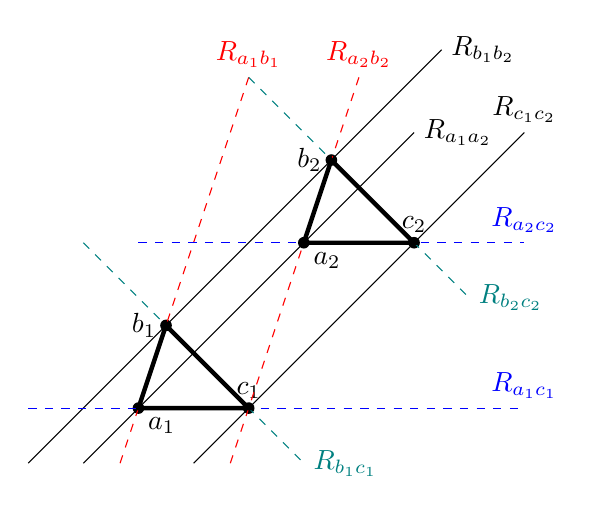
\begin{tikzpicture}[scale=0.7]
                % Los puntos del triángulo 1
                \coordinate (a_1) at (-2,0);
                \coordinate (b_1) at (-1.5,1.5);
                \coordinate (c_1) at (0,0);
    
                % Los puntos del triángulo 2
                \coordinate (a_2) at (1,3);
                \coordinate (b_2) at (3,3);
                \coordinate (c_2) at (1.5,4.5);
    
                % Las rectas que unen los triángulos
                \coordinate (R_a1a2_ini) at (-3,-1);
                \coordinate (R_a1a2_fin) at (3,5);
    
                \coordinate (R_c1c2_ini) at (-1,-1);
                \coordinate (R_c1c2_fin) at (5,5);
    
                \coordinate (R_b1b2_ini) at (-4,-1);
                \coordinate (R_b1b2_fin) at (3.5,6.5);
    
                % Las rectas que unen los vértices del triángulo 1
                \coordinate (R_a1b1_ini) at (-7/3,-1);
                \coordinate (R_a1b1_fin) at (0,6);
    
                \coordinate (R_a1c1_ini) at (-4,0);
                \coordinate (R_a1c1_fin) at (5,0);
    
                \coordinate (R_b1c1_ini) at (-3,3);
                \coordinate (R_b1c1_fin) at (1,-1);
    
                % Las rectas que unen los vértices del triángulo 2
                \coordinate (R_a2b2_ini) at (-1/3,-1);
                \coordinate (R_a2b2_fin) at (2,6);
    
                \coordinate (R_a2c2_ini) at (-2,3);
                \coordinate (R_a2c2_fin) at (5,3);
    
                \coordinate (R_b2c2_ini) at (0,6);
                \coordinate (R_b2c2_fin) at (4,2);
    
                % Dibujamos los puntos del triángulo 1
                \fill (a_1) circle (3pt) node [below right] {$a_1$};
                \fill (b_1) circle (3pt) node [left] {$b_1$};
                \fill (c_1) circle (3pt) node [above] {$c_1$};
    
                % Dibujamos los puntos del triángulo 2
                \fill (a_2) circle (3pt) node [below right] {$a_2$};
                \fill (b_2) circle (3pt) node [above] {$c_2$};
                \fill (c_2) circle (3pt) node [left] {$b_2$};
    
                % Dibujamos las rectas que unen los triángulos
                \draw[] (R_a1a2_ini) -- (R_a1a2_fin) node [right] {$R_{a_1a_2}$};
                \draw[] (R_b1b2_ini) -- (R_b1b2_fin) node [right] {$R_{b_1b_2}$};
                \draw[] (R_c1c2_ini) -- (R_c1c2_fin) node [above] {$R_{c_1c_2}$};
    
                % Dibujamos las rectas que unen los vértices del triángulo 1
                \draw[dashed, red] (R_a1b1_ini) -- (R_a1b1_fin) node [above] {$R_{a_1b_1}$};
                \draw[dashed, blue] (R_a1c1_ini) -- (R_a1c1_fin) node [above] {$R_{a_1c_1}$};
                \draw[dashed, teal] (R_b1c1_ini) -- (R_b1c1_fin) node [right] {$R_{b_1c_1}$};
    
                % Dibujamos las rectas que unen los vértices del triángulo 2
                \draw[dashed, red] (R_a2b2_ini) -- (R_a2b2_fin) node [above] {$R_{a_2b_2}$};
                \draw[dashed, blue] (R_a2c2_ini) -- (R_a2c2_fin) node [above] {$R_{a_2c_2}$};
                \draw[dashed, teal] (R_b2c2_ini) -- (R_b2c2_fin) node [right] {$R_{b_2c_2}$};
    
                % Dibujamos los triángulos
                \draw[ultra thick] (a_1) -- (b_1) -- (c_1) -- cycle;
                \draw[ultra thick] (a_2) -- (b_2) -- (c_2) -- cycle;
            \end{tikzpicture}
            \caption{\centering Rectas paralelas.}
        \end{subfigure}
        \caption{\centering Representación gráfica del Teorema de Desargues.}
    \end{figure}
\end{teo}
\begin{proof}
    Consideramos en primer lugar la traslación según el vector
    $\vec{a_1a_2}$, que como los triángulos no tienen vértices comunes, no es nulo. Sea esta traslación $t_{\vec{a_1a_2}}$.

    Como $R_{a_1b_1}\|R_{a_2b_2}$, tenemos que $\vec{a_2b_2}=\lm \vec{a_1b_1}$, para cierto $\lm\in \bb{R}$.
    Además, como $a_2\neq b_2$, tenemos que $\lm\neq 0$. Consideramos la
    homotecia de centro $a_2$ y razón $\lm$, notada por $H_{a_2, \lm}$.\\

    Sea ahora la aplicación $f=H_{a_2, \lm}\circ t_{\vec{a_1a_2}}$, que sabemos que es afín con lineal sociada:
    \begin{equation*}
        \vec{f} = \vec{H_{a_2, \lm}}\circ \vec{t_{\vec{a_1a_2}}} = \lm Id \circ Id = \lm Id
    \end{equation*}
    Por tanto, $f$ es una dilatación, por lo que transforma rectas en rectas paralelas. Notemos además que:
    \begin{align*}
        f(a_1) &= H_{a_2, \lm}(t_{\vec{a_1a_2}}(a_1)) = H_{a_2, \lm}(a_2) = a_2\\
        f(b_1) &= H_{a_2, \lm}(t_{\vec{a_1a_2}}(b_1)) = H_{a_2, \lm}(b_1+\vec{a_1a_2})
                = a_2+\lm \left(\vec{a_2\left(b_1+\vec{a_1a_2}\right)}\right) = \\
               &\qquad = a_2+\lm \left(\vec{b_1-a_2+\vec{a_1a_2}}\right)
               = a_2+\lm \left({\vec{a_2b_1}+\vec{a_1a_2}}\right) =\\
               &\qquad = a_2+\lm {\vec{a_1b_1}} \AstIg a_2 + \vec{a_2b_2} = b_2\\
        f(c_1) &= c_2
    \end{align*}
    donde en $(\ast)$ hemos usado que $\lm \vec{a_1b_1}=\vec{a_2b_2}$. Veamos ahora por qué $f(c_1)=c_2$.

    Partiendo de que $f$ lleva rectas en rectas paralelas,
    como $R_{a_1c_1}\|R_{a_2c_2}$ y $f(a_1)=a_2$, tenemos que $f(c_1)\in R_{a_2c_2}$.
    Análogamente, como $R_{b_1c_1}\|R_{b_2c_2}$ y $f(b_1)=b_2$, tenemos que $f(c_1)\in R_{b_2c_2}$. Por tanto,
    \begin{equation*}
        f(c_1)\in R_{a_2c_2}\cap R_{b_2c_2} \AstIg \{c_2\}
    \end{equation*}
    donde en $(\ast)$ hemos usado que, como $a_2\neq b_2$ por ser un triángulo, $R_{a_2c_2}$ y $R_{b_2c_2}=\{c_2\}$ no son coincidentes.
    
    En resumen, hemos visto que:
    \begin{equation*}
        f(a_1)=a_2 \qquad f(b_1)=b_2 \qquad f(c_1)=c_2
    \end{equation*}
    
    Distinguimos ahora según los valores de $\lm\in \bb{R}^\ast$:
    \begin{itemize}
        \item $\lm=1$. En este caso, $f$ es una traslación según un vector $v\in \vec{\cc{A}}$. Tenemos que:
        \begin{align*}
            f(a_1) &= a_2 = a_1 + v \Longrightarrow v = \vec{a_1a_2} \\
            f(b_1) &= b_2 = b_1 + v \Longrightarrow v = \vec{b_1b_2} \\
            f(c_1) &= c_2 = c_1 + v \Longrightarrow v = \vec{c_1c_2}
        \end{align*}

        Por tanto, tenemos que:
        \begin{equation*}
            \vec{R_{a_1a_2}} = \vec{R_{b_1b_2}} = \vec{R_{c_1c_2}} = \cc{L}\{v\}
        \end{equation*}

        Quedando así demostrado que $R_{a_1a_2}$, $R_{b_1b_2}$ y $R_{c_1c_2}$ son paralelas.

        \item $\lm\neq 0,1$. En este caso, $f$ es una homotecia, y $\exists! o\in \cc{A}$ tal que $f(o)=o$. Tenemos que:
        \begin{align*}
            f(R_{a_1a_2}) &= f\left(a_1 + \vec{R_{a_1a_2}}\right) = f(a_1) + \vec{f}\left(\vec{R_{a_1a_2}}\right) = a_2 + \lm \vec{R_{a_1a_2}} = R_{a_2a_1} \\
            f(R_{b_1b_2}) &= f\left(b_1 + \vec{R_{b_1b_2}}\right) = f(b_1) + \vec{f}\left(\vec{R_{b_1b_2}}\right) = b_2 + \lm \vec{R_{b_1b_2}} = R_{b_2b_1} \\
            f(R_{c_1c_2}) &= f\left(c_1 + \vec{R_{c_1c_2}}\right) = f(c_1) + \vec{f}\left(\vec{R_{c_1c_2}}\right) = c_2 + \lm \vec{R_{c_1c_2}} = R_{c_2c_1}
        \end{align*}

        Veamos ahora que, para toda recta $R\subset \cc{A}$ tal que $f(R)=R$, se tiene que el centro de la homotecia $o\in R$. Para todo $p\in \cc{A}$, tenemos que:
        \begin{equation*}
            f(p) = f\left(o+\vec{op}\right) = f(o) + \vec{f}\left(\vec{op}\right) = o + \lm \vec{op}
            = o + \vec{op} + (\lm-1)\vec{op} = p + (\lm-1)\vec{op}
        \end{equation*}
        Supongamos ahora que $p\in R$, luego $f(p)\in f(R)=R$.
        Por tanto, se tiene que $\vec{pf(p)}=(\lm -1)\vec{op}\in \vec{R}$, y como $\lm\neq 1$ y $p\in R$, tenemos que $o\in R$.

        Por tanto, como hemos visto que $R_{a_1a_2}$, $R_{b_1b_2}$ y $R_{c_1c_2}$ son fijas por $f$, tenemos que:
        \begin{equation*}
            o\in R_{a_1a_2} \cap R_{b_1b_2} \cap R_{c_1c_2}
        \end{equation*}

        Queda así demostrado que $R_{a_1a_2}\cap R_{b_1b_2} \cap R_{c_1c_2}=\{o\}$; es decir, son secantes en el mismo punto centro de la homotecia.


    

    \end{itemize}
    
\end{proof}

Gráficamente, el Teorema de Desargues se puede ver en el siguiente applet de Geogebra: 
\href{https://www.geogebra.org/classic/k3vvkyx9}{https://www.geogebra.org/classic/k3vvkyx9}.






\section{Convexidad}
Introducimos ahora el concepto de convexidad, que nos será de gran utilidad para definir la envolvente convexa de un conjunto de puntos.
La convexidad se estudiará en otras asignaturas, como Topología I o Análisis Matemático I.
\begin{definicion}[Segmento]
    Sea $\cc{A}$ un espacio afín. Entonces, dados dos puntos $p,q\in \cc{A}$, se define el segmento entre los puntos $p,q$ como:
    \begin{equation*}
        [p,q]=\{p+t\vec{pq}\mid t\in [0,1]\}=\{q+t\vec{qp}\mid t\in [0,1]\}
    \end{equation*}
\end{definicion}

\begin{definicion}
    Sea $\cc{A}$ un espacio afín, y $B\subset \cc{A}$. Decimos que $B$ es convexo si:
    \begin{equation*}
        [p,q]\subset B \qquad \forall p,q\in B
    \end{equation*}
\end{definicion}

Notemos que la unión de dos convexos no tiene por qué ser convexa. No obstante, sí que se cumple la siguiente propiedad:
\begin{prop}
    Sea $\cc{A}$ un espacio afín, y $\{X_i\}_{i\in I}$ convexos, con $X_i\subset \cc{A}~\forall i\in I$. Entonces, se tiene que:
    \begin{equation*}
        \bigcap_{i\in I}X_i \neq \emptyset \Longrightarrow \bigcap_{i\in I}X_i \text{ es convexo}
    \end{equation*}
\end{prop}
\begin{proof}
    Sea $p,q\in \bigcap_{i\in I}X_i$. Entonces, $p,q\in X_i~\forall i\in I$. Como $X_i$ es convexo, tenemos que $[p,q]\subset X_i~\forall i\in I$.
    Por tanto, $[p,q]\subset \bigcap_{i\in I}X_i$.
\end{proof}

Es evidente que todo espacio afín $\cc{A}$ es convexo, ya que $[p,q]\subset \cc{A}~\forall p,q\in \cc{A}$.
Además, como todo subespacio afín es un espacio afín, tenemos que todo subespacio afín es convexo.

Respecto a las aplicaciones afines, tenemos los siguientes resultados:
\begin{prop}
    Sean $\cc{A},\cc{A}'$ espacios afines, y sea $f:\cc{A}\to \cc{A}'$ una aplicación afín. Entonces, se tiene que:
    \begin{enumerate}
        \item $f([p,q])=[f(p),f(q)]$ \qquad $\forall p,q\in \cc{A}$.
        \item Si $B\subset \cc{A}$ es convexo, entonces $f(B)\subset \cc{A}'$ es convexo.
        \item Si $B'\subset \cc{A}'$ es convexo y $f^{-1}(B')\neq \emptyset$, entonces $f^{-1}(B')$ es convexo.
    \end{enumerate}
\end{prop}
\begin{proof}
    Demostramos cada resultado por separado:
    \begin{enumerate}
        \item Sea $p,q\in \cc{A}$. Entonces, tenemos que:
        \begin{equation*}
            \begin{split}
                f([p,q]) &= f(\{p+t\vec{pq}\mid t\in [0,1]\}) = \{f(p+t\vec{pq})\mid t\in [0,1]\} =\\&= \{f(p)+t\vec{f}(\vec{pq})\mid t\in [0,1]\}
            = \{f(p)+t\vec{f(p)f(q)}\mid t\in [0,1]\} = [f(p),f(q)]
            \end{split}
        \end{equation*}
        donde he aplicado que $f$ es afín, y por tanto, $\vec{f}(\vec{pq})=\vec{f(p)f(q)}$.

        \item Sean $p',q'\in f(B)$. Entonces, $\exists p,q\in B$ tales que $f(p)=p', f(q)=q'$.
        
        Como $B$ es convexo, tenemos que $[p,q]\subset B$. Por tanto, $f([p,q])\subset f(B)$. Además, por el apartado anterior, $f([p,q])=[f(p),f(q)]=[p',q']$. Por tanto, $[p',q']\subset f(B)$, por lo que $f(B)$ es convexo.

        \item Sean $p,q\in f^{-1}(B')$. Entonces, $f(p),f(q)\in B'$, por lo que $[f(p),f(q)]\subset B'$. Por tanto, $f([p,q])\subset B'$, por lo que $[p,q]\subset f^{-1}(B')$.
    \end{enumerate}
\end{proof}


\subsection{Envolvente convexa}
Introducimos ahora el concepto de envolvente convexa:
\begin{definicion}[Envolvente convexa]
    Sea $\cc{A}$ un espacio afín, y $B\subset \cc{A}$. Definimos la envolvente convexa de $B$ como el menor subconjunto convexo que contiene a $B$. Es decir,
    \begin{equation*}
        \varphi(B)=\bigcap \{X\supset B\mid X\text{ es convexo}\}
    \end{equation*}
\end{definicion}

Algunas propiedades de la envolvente convexa son:
\begin{enumerate}

    \item $B\subset \varphi(B)$ \qquad $\forall B\subset \cc{A}$.
    \item $\varphi(\varphi(B))=\varphi (B)$ \qquad $\forall B\subset \cc{A}$.
    
    Esto se tiene de forma directa, ya que $\varphi(B)$ es convexo.

    \item $X\subset Y \Longrightarrow \varphi(X)\subset \varphi(Y)$ \qquad $\forall X,Y\subset \cc{A}$.
    
    Esto se tiene de forma directa también, ya que $\varphi(Y)$ es convexo y $X\subset Y\subset \varphi(Y)$, por lo que $\varphi(X)\subset \varphi(Y)$.

    \item $\varphi (X)\cup \varphi (Y)\subset \varphi (X\cup Y)$ \qquad $\forall X,Y\subset \cc{A}$.
    
    En primer lugar, tenemos que $X \subset X\cup Y$, por lo que $\varphi(X)\subset \varphi(X\cup Y)$. Análogamente, $\varphi(Y)\subset \varphi(X\cup Y)$. Por tanto, $\varphi(X)\cup \varphi(Y)\subset \varphi(X\cup Y)$.
\end{enumerate}

Notemos que $\varphi(X)\cap \varphi(Y)$ no tiene por qué ser igual a $\varphi(X\cap Y)$.
\begin{ejemplo}
    Algunos ejemplos de envolvente convexa son:
    \begin{enumerate}
        \item Para $B=\{p\}$, tenemos que $\varphi(B)=\{p\}$.
        \item Para $B=\{p,q\}$, tenemos que $\varphi(B)=[p,q]$.
        \item Para $B=\{p,q,r\}$ no alineados, tenemos que $\varphi(B)$ es el triángulo formado por los puntos $p,q,r$, junto con su interior.
    \end{enumerate}
\end{ejemplo}

\section{Relación de Ejercicios}

Para ver ejercicios relacionados con este tema, consultar la sección \ref{Rel:Tema1}.